\documentclass[a4paper, 12pt, openany, oneside]{jsbook}

\usepackage[dvipdfmx]{graphicx}
\usepackage[dvipdfmx]{color}
\usepackage[dvipdfmx, bookmarks=true, setpagesize=false]{hyperref}
\usepackage{pxjahyper}
\usepackage[hang,small,bf]{caption}
\usepackage[subrefformat=parens]{subcaption}
\captionsetup{compatibility=false}

\usepackage{thesis}
\usepackage{here}
\usepackage{url}


\thesis{卒 業 論 文}
\title{
  \centering
    \scalebox{1.0}{視覚と行動の end-to-end 学習により経路追従行動を}\\
    \vspace{-0.3zh}
    \scalebox{1.0}{オンラインで模倣する手法の提案}\\
    \vspace{-0.3zh}
    \scalebox{1.0}{(目標方向による経路選択機能の追加)}\\
    \vspace{0.4zh}
    \scalebox{0.7}{A proposal for an online imitation method of path-tracking}
    \vspace{-0.7zh}
    \scalebox{0.7}{behavior by end-to-end learning of vision and action}\\
    \vspace{0.5zh}
    \scalebox{0.7}{(Addition of path selection function by target direction)}
    \vspace{-7.0zh}
}
\setlength{\textwidth}{\fullwidth}
\setlength{\evensidemargin}{\oddsidemargin}

\date{\today}
\vspace{-15.0zh}
\teacher{林原 靖男 教授}
\vspace{-15.0zh}
\organization{千葉工業大学 先進工学部 未来ロボティクス学科}
\author{18C1096 春山 健太}
\vspace{-15zh}

\renewcommand{\baselinestretch}{1.2}
\begin{document}

%% Front Matter
\frontmatter{}
%
\maketitle
%
%!TEX root = ../thesis.tex
\chapter*{概要}
\thispagestyle{empty}
%
\begin{center}
  \scalebox{1.5}{カメラ画像と目標方向を用いたend-end学習による}\\
  \scalebox{1.5}{分岐路でのルート選択可能なのnavigation手法の提案}\\
\end{center}
\vspace{1.0zh}
%

近年,カメラ画像に基づいた自律移動の研究が行われている.
本研究室でも,LiDAR を用いた自律移動システムの出力を教師信号として与えることで
ロボットの経路追従行動をオンラインで模倣する手法を提案し,
実験により一定の経路を周回可能であると示されている.
本研究では,従来手法をベースに,目標とする進行方向("目標方向")をデータセットと学習器の入力へ加えることで,
分岐路で「直進」と「左折」などの経路を選択可能とする機能の追加を提案する.
提案手法では,LiDAR を用いた自律移動システムの出力をカメラ画像と目標方向を用いて模倣学習し,
学習後,カメラ画像と目標方向に基づいて経路を選択可能な自律走行を行う.
また,シミュレータを用いた実験により,提案手法の有効性を検証した. 

キーワード: end-to-end学習, Navigation, 目標方向
%
\newpage
%%
\chapter*{abstract}
\thispagestyle{empty}
%
\begin{center}
  \scalebox{1.3}{An End-to-End Navigation Method for Route Selection on Branch Roads}
  \scalebox{1.3}{Using Camera Images and Target Directions}\\
\end{center}
\vspace{1.0zh}
%

In recent years, research on autonomous mobility based on camera images has been conducted.
In our laboratory, we have proposed a method to imitate the path-following behavior of a robot online by providing the output of a LiDAR-based autonomous mobility system as a supervisory signal. I have also proposed a method to imitate the robot's path-following behavior online by providing the output of a LiDAR-based autonomous moving system as a supervisory signal, Experiments have shown that it is possible to follow a certain path.
In this study, based on the conventional method, I propose a method to imitate a robot's path-following behavior by adding a target direction ("target direction") to the data set and the input of the learner. 
In this paper, I propose to add a function that allows the user to select a path such as "straight ahead" or "left turn" at a forked road by adding the target direction ("target direction") to the dataset and the input of the learner.
The proposed method imitates and learns the output of a LiDAR-based autonomous mobility system using camera images and target directions.
After learning, the system runs autonomously and can select a route based on the camera image and the target direction.
I also verified the effectiveness of the proposed method by experiments using a simulator. 


keywords: End-to-end Learning, Navigation, Target Direction

%
\tableofcontents
%
\listoffigures
%
\listoftables
%

%
%% Main Matter
\mainmatter{}

\chapter{序論}
\section{背景}
近年,様々なセンサを用いた移動ロボットの自律移動に関する研究が盛んに行われており,
その中でカメラ画像を用いてロボットへ自律移動を行わせる研究も行われている.
%\index{うえだ@上田}
%例として,\cite{上田2015gihyo,ueda2015,上田2015jsai}がある.
Bojaskiら\cite{Nvidia}は
Fig. \ref{fig::nvidia}で示す方法で,人間のハンドル操作によるステアリングの角度の模倣学習を行い,
画像を用いて走行を行う方法を提案した.

\begin{figure}[h]
    \centering
    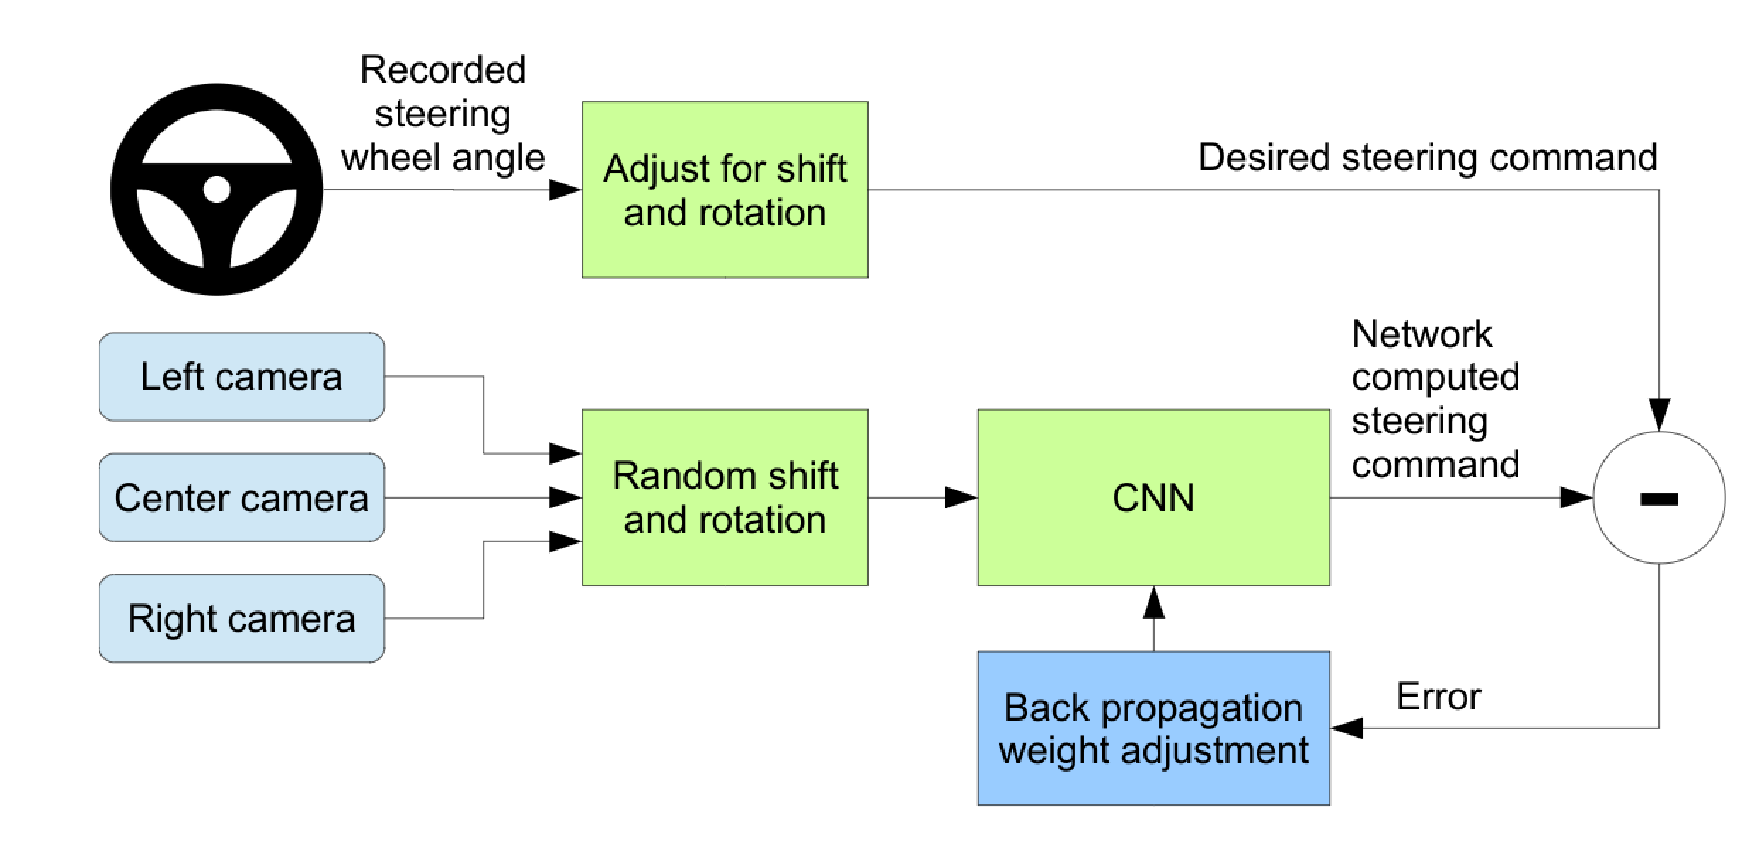
\includegraphics[width = 13cm]{./figs/EndtoEnd_Learning_for_Self-Driving_Cars.pdf}
    \caption{Training the neural network from \cite{Nvidia}}
    \label{fig::nvidia}
\end{figure}

\newpage
本研究室においても岡田ら\cite{okada}によってFig. \ref{fig::okada_sys}に示すシステム
LiDAR,オドメトリなどの入力としたルールべースの制御器の出力による自律走行を行い
その際にロボットから取得したカメラ画像を入力,ルールベース制御器の出力した角速度を目標出力として学習器の訓練を行い,
訓練後にはカメラ画像を入力を学習器へ入力し,その出力を用いて走行を行う
ルールベース制御器を用いてデータセット収集における労力の削減と経路へ戻る行動が学習可能な
Fig.\ref{fig::okada}で示すルールベース制御器の経路追従行動を模倣する手法が提案されている.
\begin{figure}[h]
    \centering
    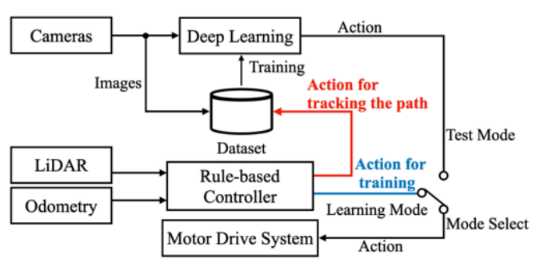
\includegraphics[width = 10cm]{./figs/okada_sys.png}
    \caption{Okada and others proposed method from \cite{okada}}
    \label{fig::okada_sys}
\end{figure}

\begin{figure}[h]
    \centering
    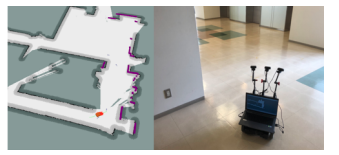
\includegraphics[width = 10cm]{./figs/okada.png}
    \caption{A robot that follows a path using vision based on the proposed method\cite{okada}}
    \label{fig::okada}
\end{figure}

\newpage
上記の研究により,カメラ画像用いてロボットが学習した経路を
周回可能であることが確認されている.


次に岡田ら\cite{okada}研究を一定の経路の周回以外への拡張について考える.
走行する経路内にFig. \ref{fig::bunki}のような分岐路が含まれる場合,
画像のみを入力としたネットワークでは,分岐路においてネットワークが2つの方向を出力してしまい,
左右に車体を向ける振動が発生してしまう事象がDean A. Pomerleauら\cite{pomeru}によって確認されている.
そのため赤と緑の矢印で示した直進と左折のようなルートを任意に切り替えを行うためには,
カメラ画像のみを入力とした場合「分岐路をどちらへ進むか」というルート選択を行うために
情報が必要だと考えられる.
 \vspace{4.0zh}
\begin{figure}[h]
    \centering
    \includegraphics[width = 8cm]{./figs/bunki.pdf}
    \caption{Cross road}
    \label{fig::bunki}
\end{figure}
\newpage

分岐路でルートを選択をする情報として
人間の交差点などの目印に基づいて目的地まで移動する能力を,
島田らは分岐路などの目印(エッジ)とそのつながり(ノード)を表現する地図(トポロジカルマップ)
Fig. \ref{fig::topo}と
次の情報を持つエッジ
1) ID
2) Type(通路の特徴)
3) Edge(エッジの ID と相対角度)
トポロジカルマップより「道案内」同様に,「次の角まで」のような「条件」と「直進」などの「行動」
の組み合わせで作成した経路の情報(シナリオ)\ref{fig::sina}
を用いて表現した自律移動ロボットのNavigation手法を提案している.

\begin{figure}[H]
    \centering
    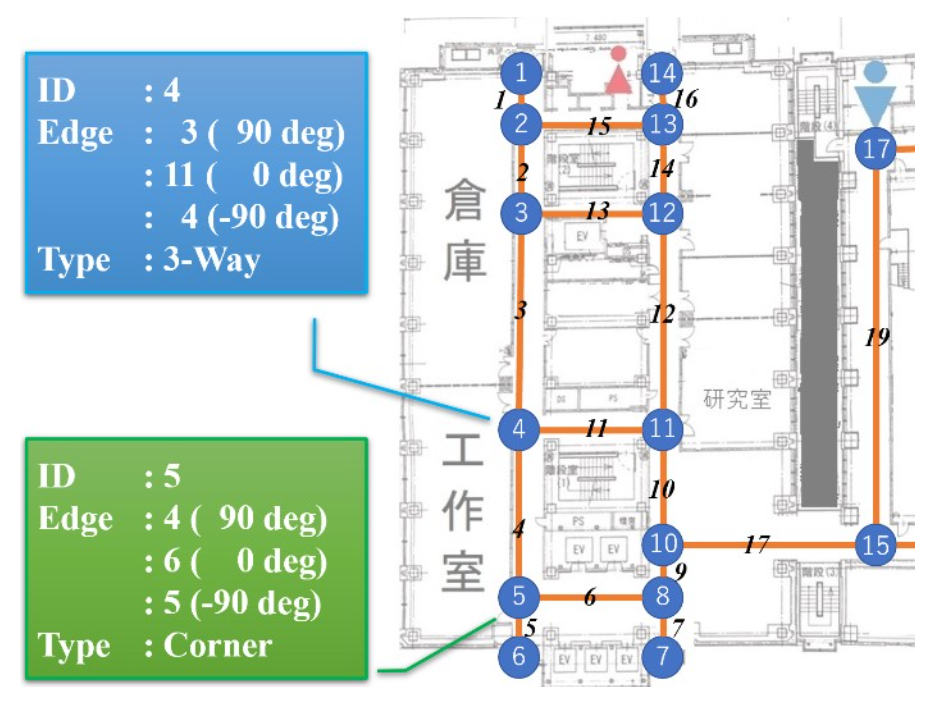
\includegraphics[width = 13cm]{./figs/topo.png}
    \caption{topo\cite{razikon}}
    \label{fig::topo}
\end{figure}
\begin{figure}[H]
    \centering
    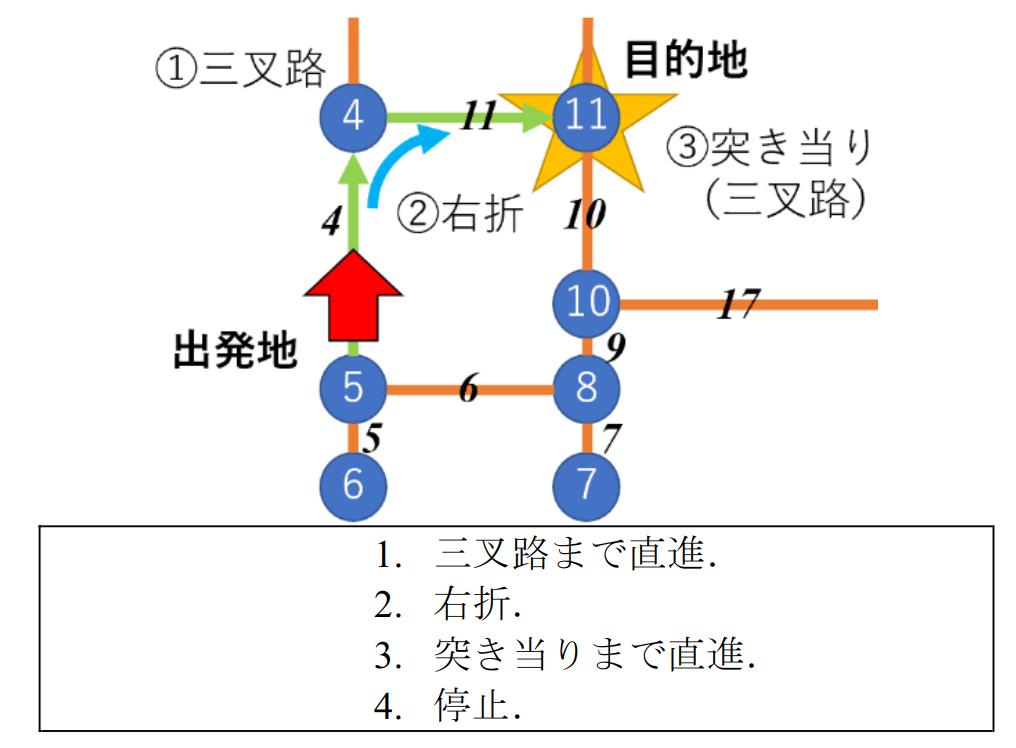
\includegraphics[width = 13cm]{./figs/sina.png}
    \caption{sina\cite{razikon}}
    \label{fig::sina}
\end{figure}

そこで本研究では,島田らが提案した「シナリオ」から生成した
「直進」「左折」「右折」などの目標とする方向の情報(本研究では"目標方向"とする)
を\cite{okada}らが提案した手法において学習器の入力へ追加し,
学習器の出力を用いた走行で分岐路において特定のルート選択を行う
「カメラ画像と目標方向を用いたEnd-to-End学習によるシナリオを用いたNavigation手法」を提案する.
提案手法全体の流れをFig. \ref{fig::haikei_zentai}に示す.
\begin{figure}[H]
    \centering
    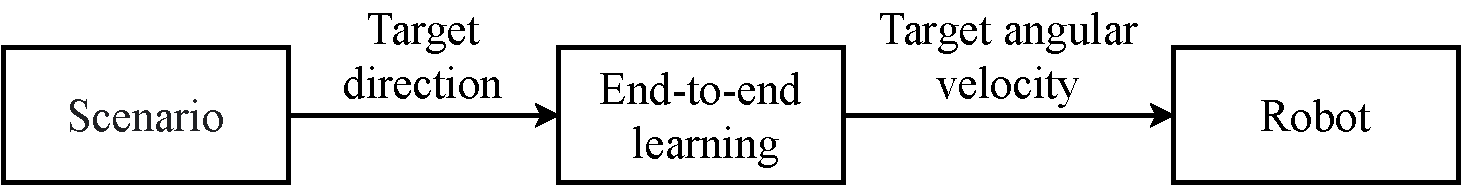
\includegraphics[width = 13cm]{./figs/haikei_zentai.pdf}
    \caption{hai}
    \label{fig::haikei_zentai}
\end{figure}

\newpage
カメラ画像と他の情報を用いて,自律移動を行う研究として
Felipeら\cite{razikon}はカメラ画像と操舵角と加速度の2次元の制御信号と,continue,left,straight,rightの4つのコマンドを入力としたネットワークを
用いてFig. \ref{fig::Conditional_Imitation_Learning}で示すように実環境と都市環境のシミュレータ上で学習器がコマンドに沿った行動が可能であることを
確認している.
\begin{figure}[H]
    \centering
    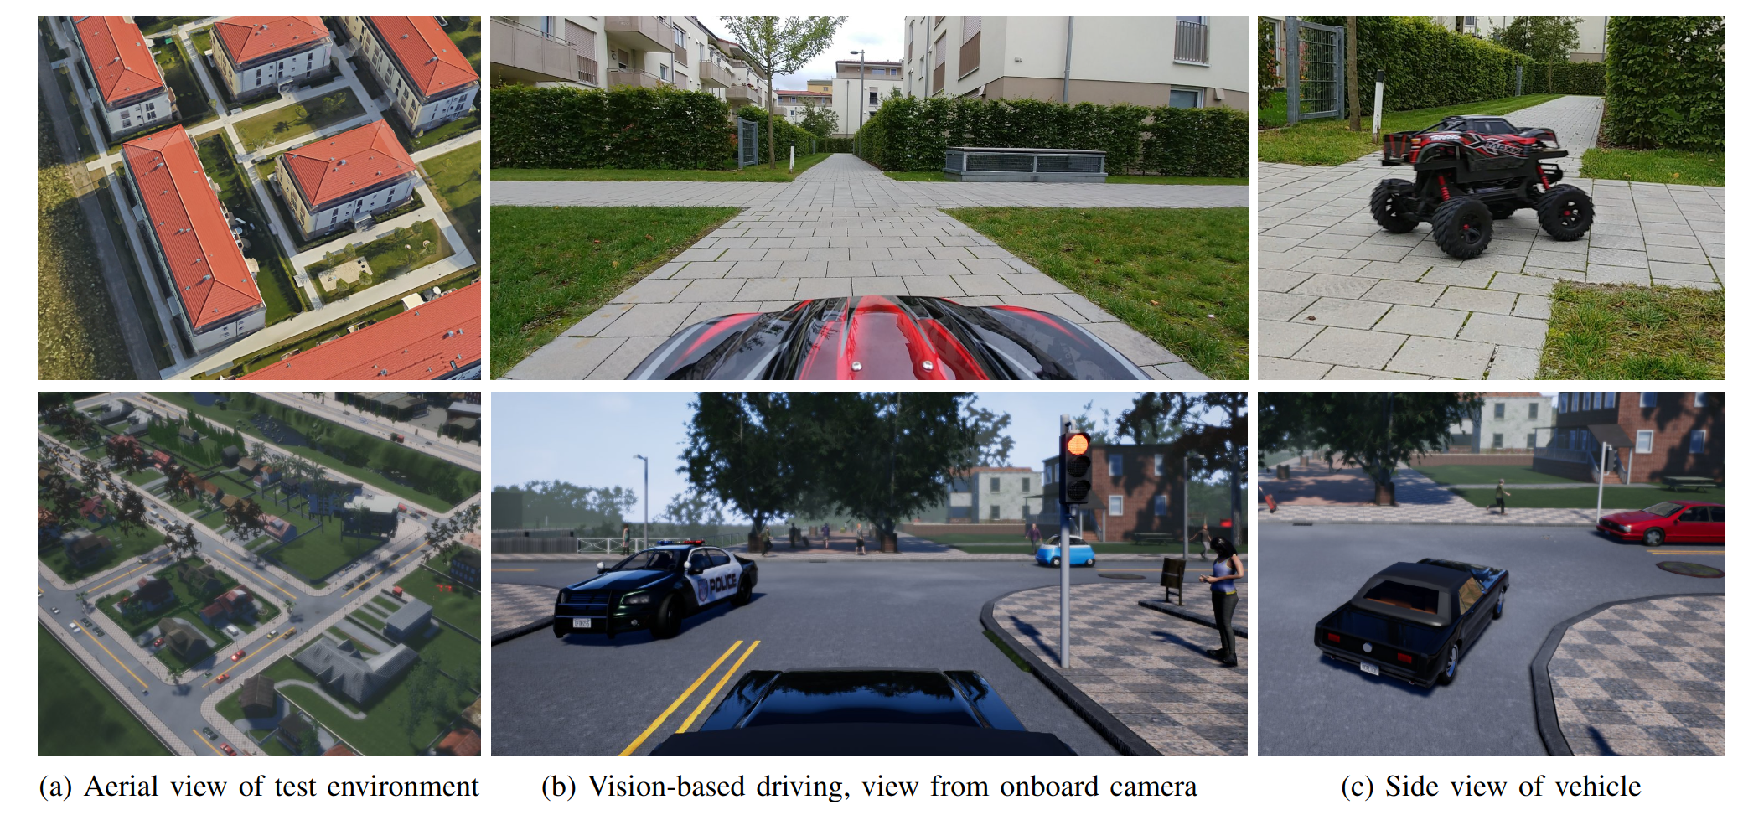
\includegraphics[width = 12cm]{./figs/End-to-end_Driving_via_Conditional_Imitation_Learning.pdf}
    \caption{End-to-end  Driving  via  Conditional  Imitation  Learning from \cite{razikon}}
    \label{fig::Conditional_Imitation_Learning}
\end{figure}

また,Seiyaら\cite{nagoya}はFig. \ref{fig::nagoyaabst}で示すように
カメラ画像と目標方向を入力,ステアリング制御信号を出力とするシステムを用いて,右および左に曲がる屋外の軌道を
追跡可能であることを確認している.

\begin{figure}[H]
    \centering
    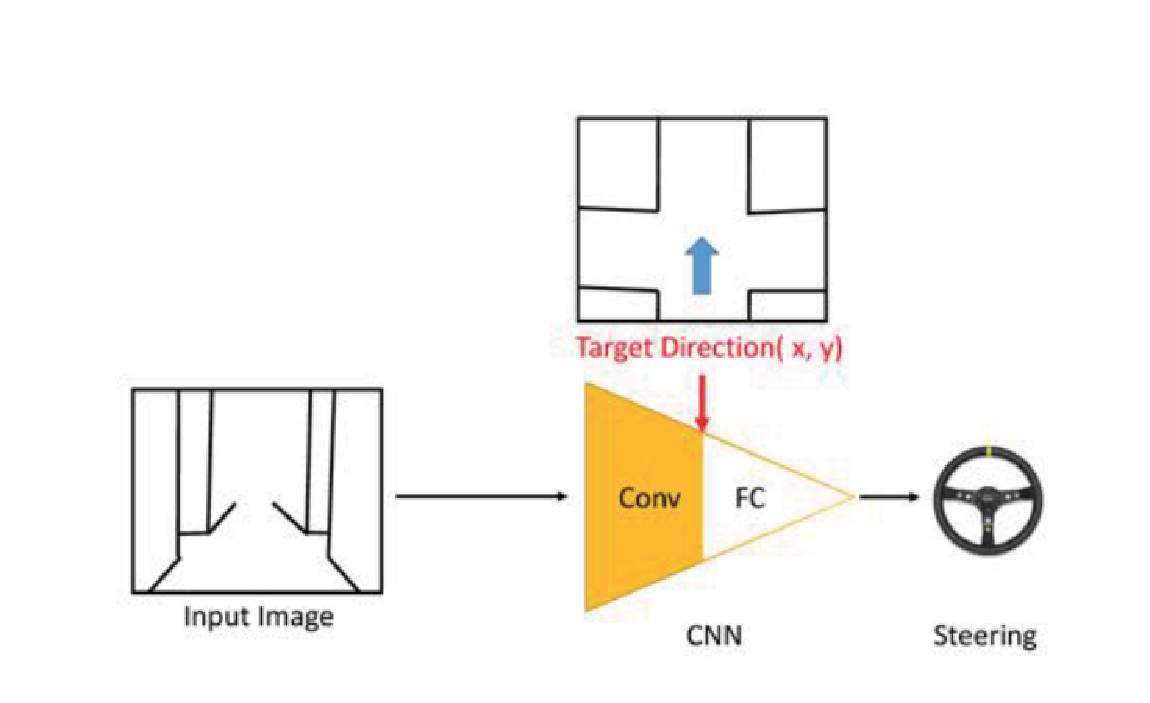
\includegraphics[width = 9.8cm]{./figs/End-to-End_Navigation_with_Branch_Turning_Support_using_Convolutional_Neural_Network_abst.pdf}
    \caption{Overview of Seiya and others proposed method from \cite{nagoya}}
    \label{fig::nagoyaabst}
\end{figure}


\section{目的}
本研究では,岡田らと島田らの研究を拡張し,
カメラ画像と目標方向を用いたEnd-to-End学習
によるシナリオに基づいたNavigation手法を行う予備段階として
Fig. \ref{fig::haikei_abs}に赤枠で示した部分を対象とする,
\begin{figure}[H]
    \centering
    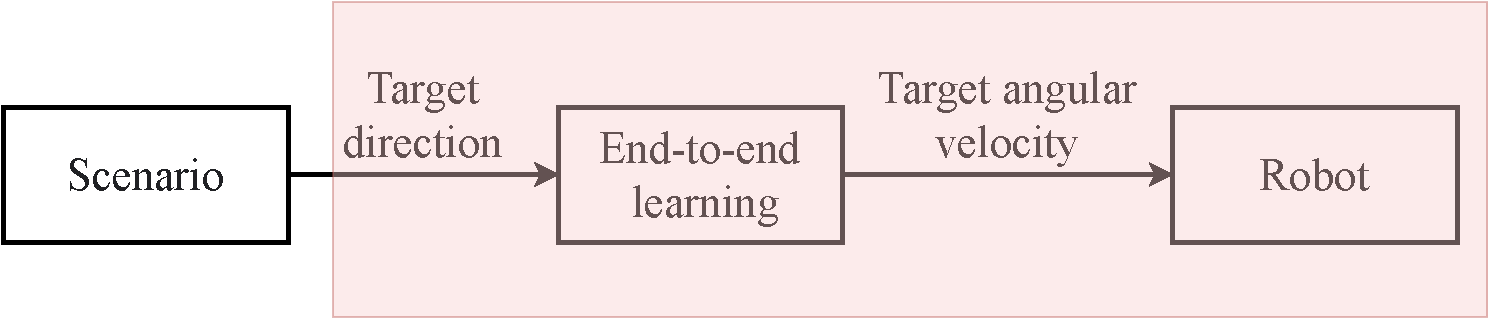
\includegraphics[width = 12cm]{./figs/haikei_abs.pdf}
    \caption{a}
    \label{fig::haikei_abs}
\end{figure}

カメラ画像と目標方向を入力とする学習器の出力を用いた走行において,
目標方向によって分岐路で任意のルートへ走行経路を変更することを目指す.
カメラ画像以外に分岐路での方向指示の情報を追加し,その情報を用いてルート選択が可能であるかの
検証を行う.


\section{論文構成}
1章では,本研究における背景,及び目的を述べた.
2章では,本研究で用いた深層学習の要素技術について述べる.
3章では,本研究で用いた手法と構築したシステムについて述べる.
4章では,構築したシステムを用いた実験を行う.
5章では,本研究の結論を述べる.

%要素技術
\chapter{要素技術}
本章では,本研究で用いた深層学習に関連した要素技術と,ベースとする従来手法について述べる.

\section{Deep learning}
Deep learningは近年,自然言語処理など様々な分野で利用されている.
人間の脳におけるニューロンの構造を数理モデル(パーセプトロン)を用いて再現したニューラルネットワークを多層構造にすることで,
複雑なタスクの解決に必要な関数の表現力を高めたものである.
一般的な構造をFig. \ref{fig::network}示す.

\begin{figure}[h]
    \centering
    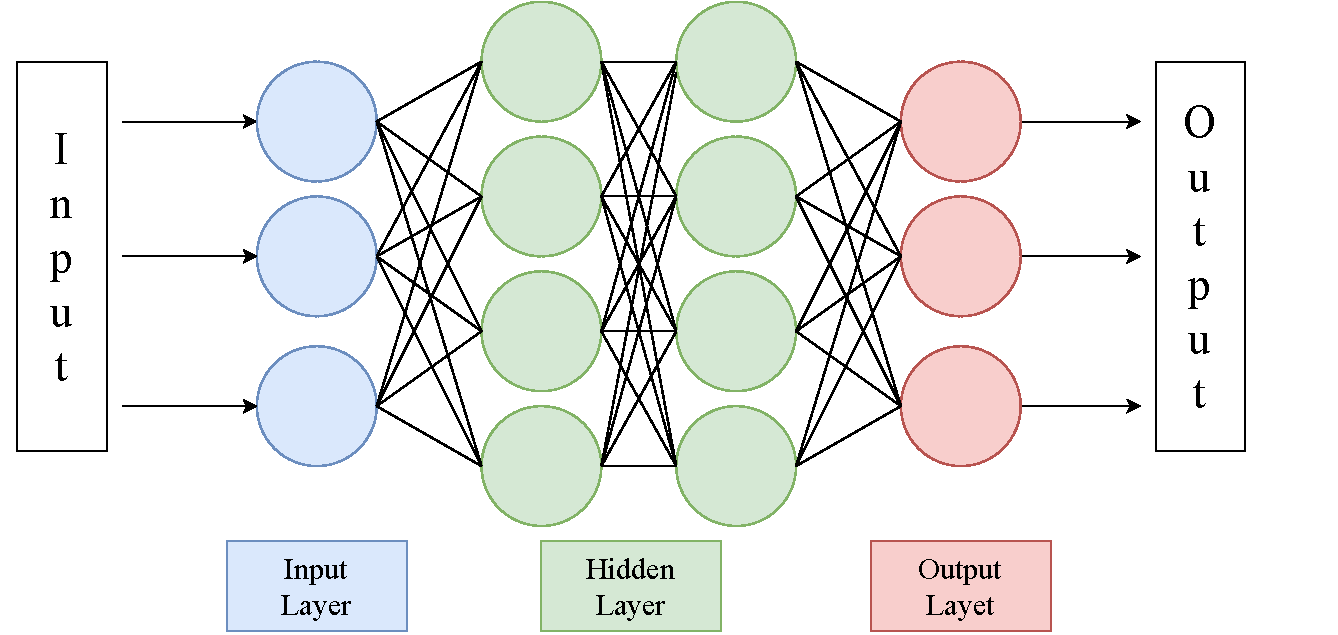
\includegraphics[width = 12cm]{./figs/net.pdf}
    \caption{Neual network}
    \label{fig::network}
\end{figure}

\section{end-to-end学習}
end-to-endとは,
Fig. \ref{fig::e2e}に示すように生データ(入力)から目的の結果(出力)を得るために必要な多段階の処理をNeusal Networkを用いて直接学習を行うものである.

実世界における自動運転を例に述べる.
人物や障害物などの物体認識,走行レーンの検出,経路計画,ステアリング制御
などの人間が設定した複数個のタスクを解く必要があるが,end-to-end学習では先程のタスクを人間が直接設定せずに
カメラ画像をニューラルネットワークに入力することで直接ステアリング操作を学習する.

\vspace{2.0zh}
\begin{figure}[h]
    \centering
    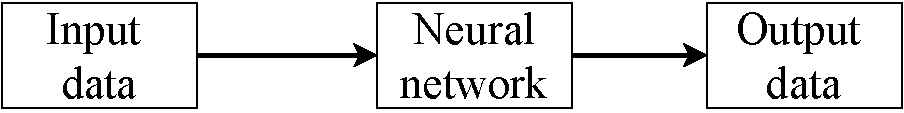
\includegraphics[width = 10cm]{./figs/e2e.pdf}
    \caption{Structure of end-to-end learning}
    \label{fig::e2e}
\end{figure}

\newpage
\section{Convolition Neual Network}
畳み込みニューラルネットワーク(convolutional neural network:CNN)は
画像認識や音声認識などの多次元の配列で表される複雑なデータを扱う処理へ用いられているニューラルネットワークである.
次のような特徴をもつ層で構成されている.

\begin{enumerate}
    \item 畳み込み層:入力データへフィルタ(カーネル)を用いて畳み込み演算を行うことで,特徴を抽出した特徴マップを取得する
    \item プーリング層:Maxプーリングなどの演算を用いて特徴マップのダウンサンプリングを行う
    \item 全結合層:畳み込み層,プーリング層で行った特徴を抽出したデータを一つのノードに
                      集約を行い,分類などの結果の出力を行う
\end{enumerate}


Krizhevskら\cite{Imagenet}はFig. \ref{fig::alex}で示すような3つの畳み込み層(convolutional layer),2つのプーリング層(pooling layer)
および 3 つの全結合層(fully connected layer)から構成したネットワークを用いて,
120万の高解像度画像を1,000の異なるクラスに分類をエラー率15.3\%で達成し,画像分類コンペティションであるILSVRC(ImageNet Large Scale Visual Recognition Competition)2012
で優勝をおさめた

\vspace{2.0zh}

\begin{figure}[h]
    \centering
    \includegraphics[width = 11.5cm]{./figs/alex.pdf}
    \caption{Alex net from \cite{Imagenet}}
    \label{fig::alex}
\end{figure}

\newpage
\section{地図ベースの制御器}
    \label{seigyo}
    従来手法と提案手法において,教師信号として用いる地図ベースの制御器について述べる.
    % 概要をFig. \ref{fig::navigation}に示す.
    地図べースの制御器は,ROS Navigation\_stack\cite{navigation:online}へ目標の経由地点(waypoint)の指示を行うwaypoint\_navを組み合わせたものである.
    ROS navigation\_stackは\ref{fig::mapbase}に示すように,事前に作成した地図とLiDAR,オドメトリを
    用いて,地図上の自己位置推定をParticle\_Filterによって確率的に行う「amcl」.
    障害物認識などの局所的または地図全体の大域的なコスト計算と,
    その結果を用いて経路計画,それに従ったモータ指令を行う「move\_base」
    などのパッケージを統合した自律走行用のメタパッケージである.
    従来手法,提案手法ではモータ指令を並進速度と角速度にわけ,並進速度は一定としている.
    % コスト計算を行うlocal\_costmapと結果を利用して,局所的な経路計画を行うlocal\_planner.
    % 地図に対して全体のコスト計算を行うglobal\_costmap,その結果を利用して大域的な経路計画を行うglobal\_plannner.
    % 「move\_base」のパッケージを統合した自律移動用のメタパッケージである.
    % 上記のと目標地点(waypoint)の指示を行う「waypoint\_nav」を組み合せることで,
    % Fig. \ref{fig::mapbase}に示す経路計画を行い,それに従ったモータ指令を行う
    
    
    % \vspace{2.0zh}
    % \begin{figure}[H]
    %     \centering
    %     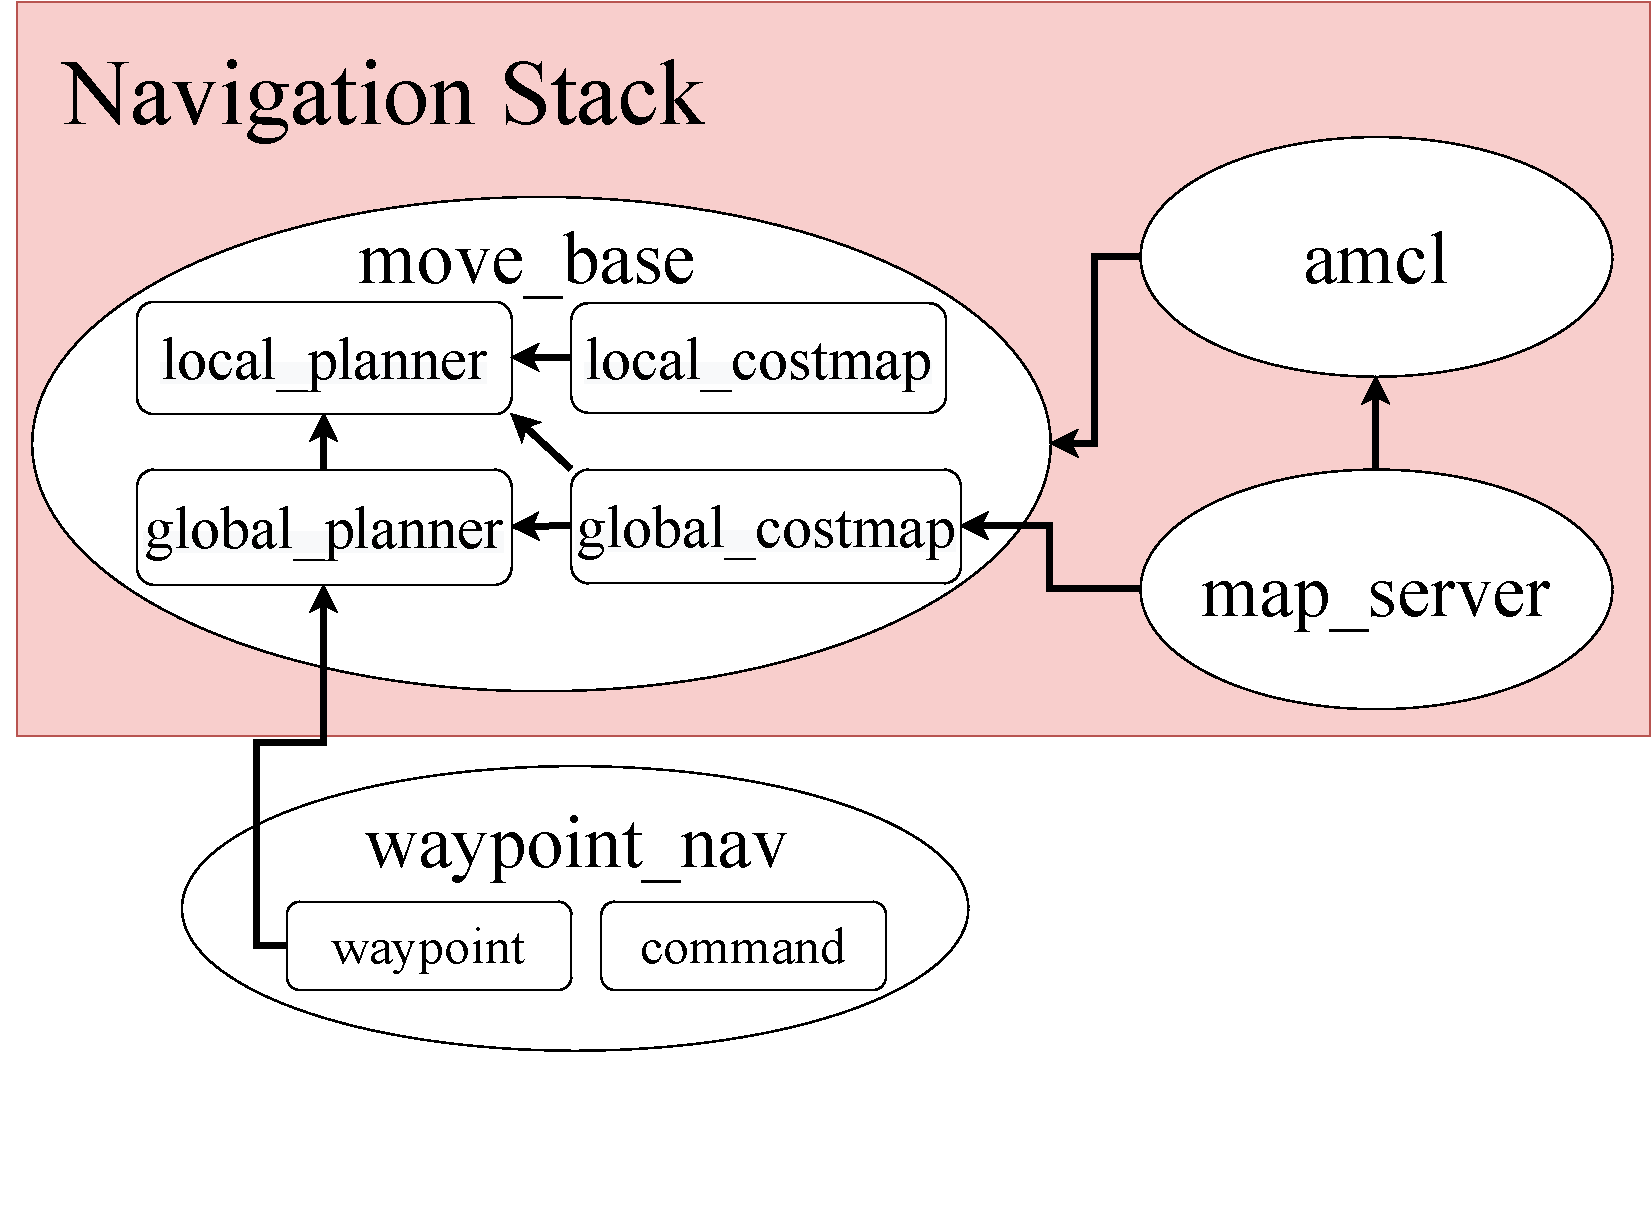
\includegraphics[width = 11cm]{./figs/navigation.pdf}
    %     \caption{Map-based controller}
    %     \label{fig::navigation}
    % \end{figure}

    \begin{figure}[H]
        \centering
        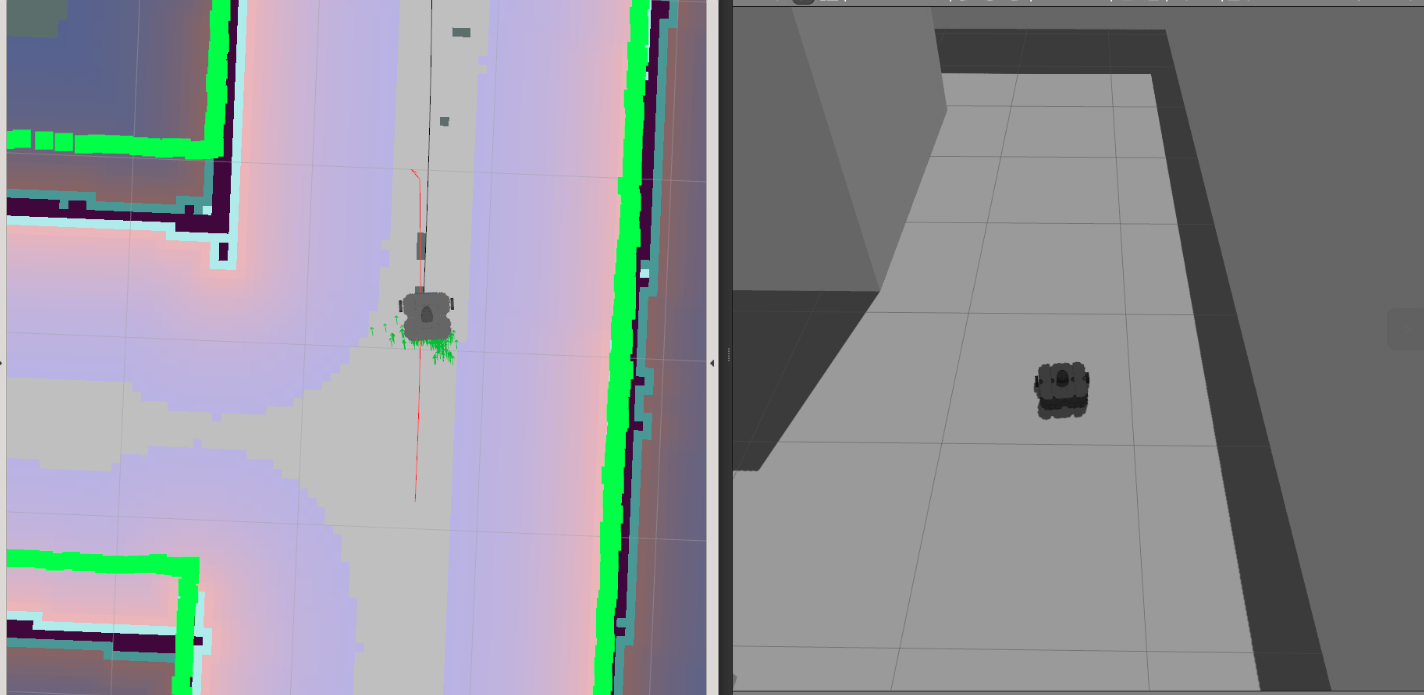
\includegraphics[width = 11cm]{./figs/mapbased.png}
        \caption{Map-based controller}
        \label{fig::mapbase}
    \end{figure}
\newpage
\section{従来手法}
本研究のベースとする岡田らの研究について述べる.
従来手法は,LiDARを用いた走行を学習し,同じ行動を画像も用いて行う手法である.
学習器の訓練を行う「学習フェーズ」と,学習器の出力を用いて走行を行う「訓練フェーズ」の2つにわけられる.
なお,2つのフェーズでの並進速度は固定した同じ値を用いる.

学習フェーズを\ref{fig::okada_method_ler}に示す.
LiDARとオドメトリを入力する地図ベースの制御器により自律移動を
カメラ画像を用いて模倣する.
学習器は入力をカメラ画像,出力を自律走行時の角速度としてend-to-end学習を行う.
\begin{figure}[h]
    \centering
    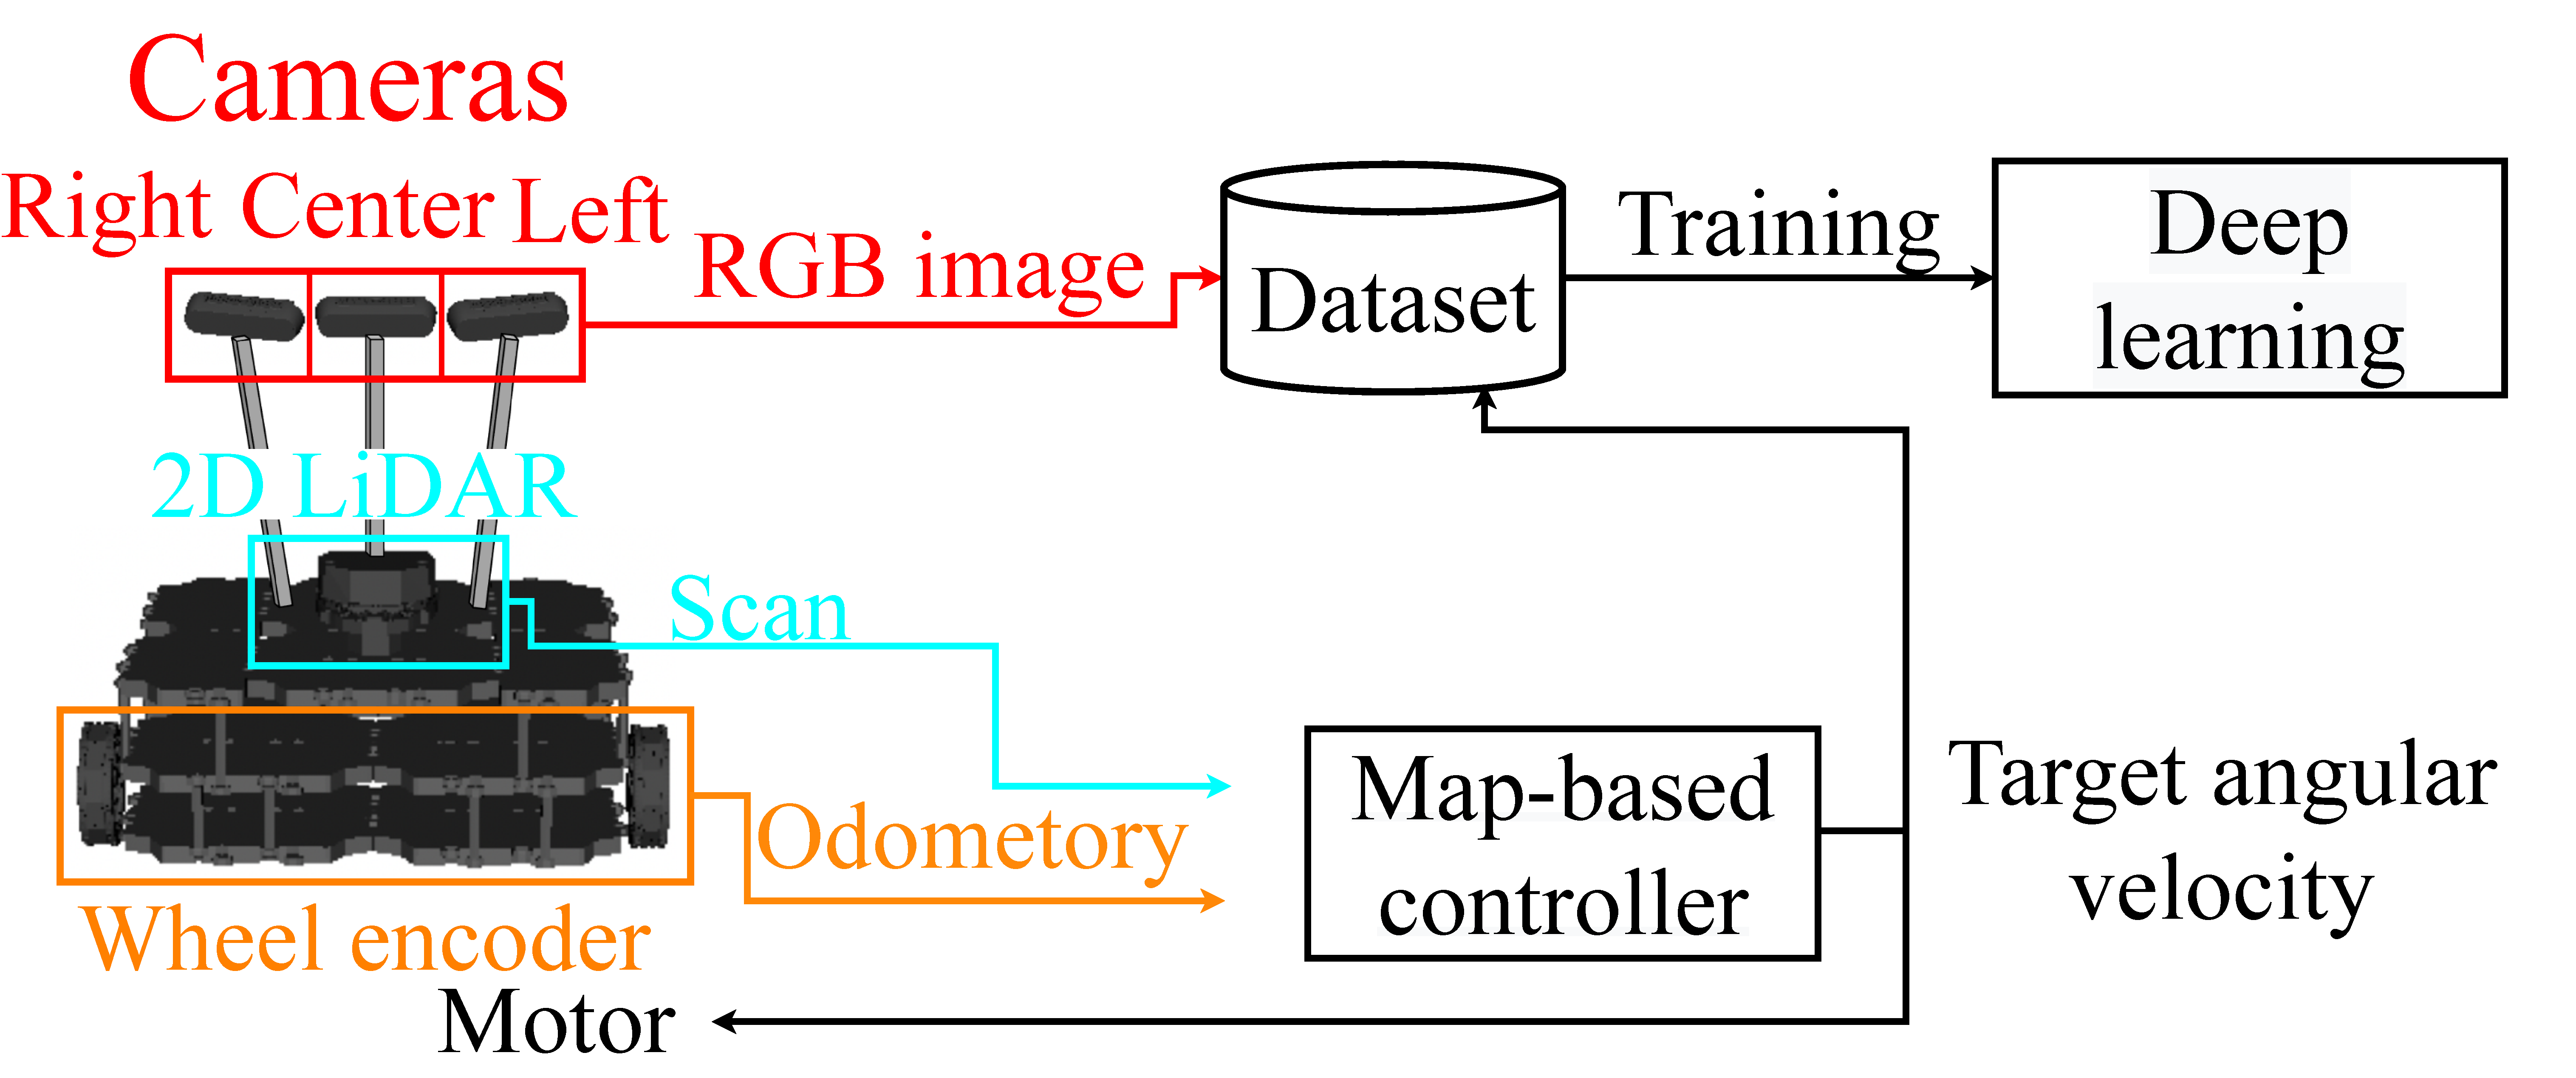
\includegraphics[width = 12cm]{./figs/system_learning_okada.pdf}
    \caption{Learning phase of conventional method}
    \label{fig::okada_method_ler}
\end{figure}

\newpage
学習フェーズでは機体の中央, 左,右に傾けて取り付けた3つのカメラを用いる.
その際,直進時に,同時に旋回のデータを取得すること及び過学習の抑制を目的として,
Table\ref{tb::camera_ang}に示すような処理を行う.
\begin{table}[H]
    \centering
    \caption{camera }
    \begin{tabular}{|c|c|ll}
    \hline
    Left camera   & Angular velocity of Map-based controller + 0.2 rad/s \\ \hline
    Center camera & Angular velocity of Map-based controller             \\ \hline
    Right camera  & Angular velocity of Map-based controller - 0.2 rad/s  \\ \hline
    \end{tabular}
    \label{tb::camera_ang}
    \end{table}
また,地図べースの制御器を教師信号とすることで,学習器の訓練に用いるデータセットと
\ref{fig::okada_path}に示すような経路へ戻る行動を自動的に収集可能としている.
\begin{figure}[h]
    \centering
    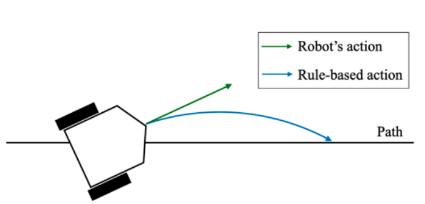
\includegraphics[width = 10cm]{./figs/okada_path.png}
    \caption{Collects the rule-based actions the robot's actions from \cite{okada}}
    \label{fig::okada_path}
\end{figure}

\newpage
学習器の訓練後,\ref{fig::okada_method_test}で示すテストフェーズへ移行する.
テストフェーズでは,カメラ画像を入力する学習器の出力する角速度を用いて自律走行を行う.
なお,テストフェーズでは中央のカメラのみを用いる.
\begin{figure}[h]
    \centering
    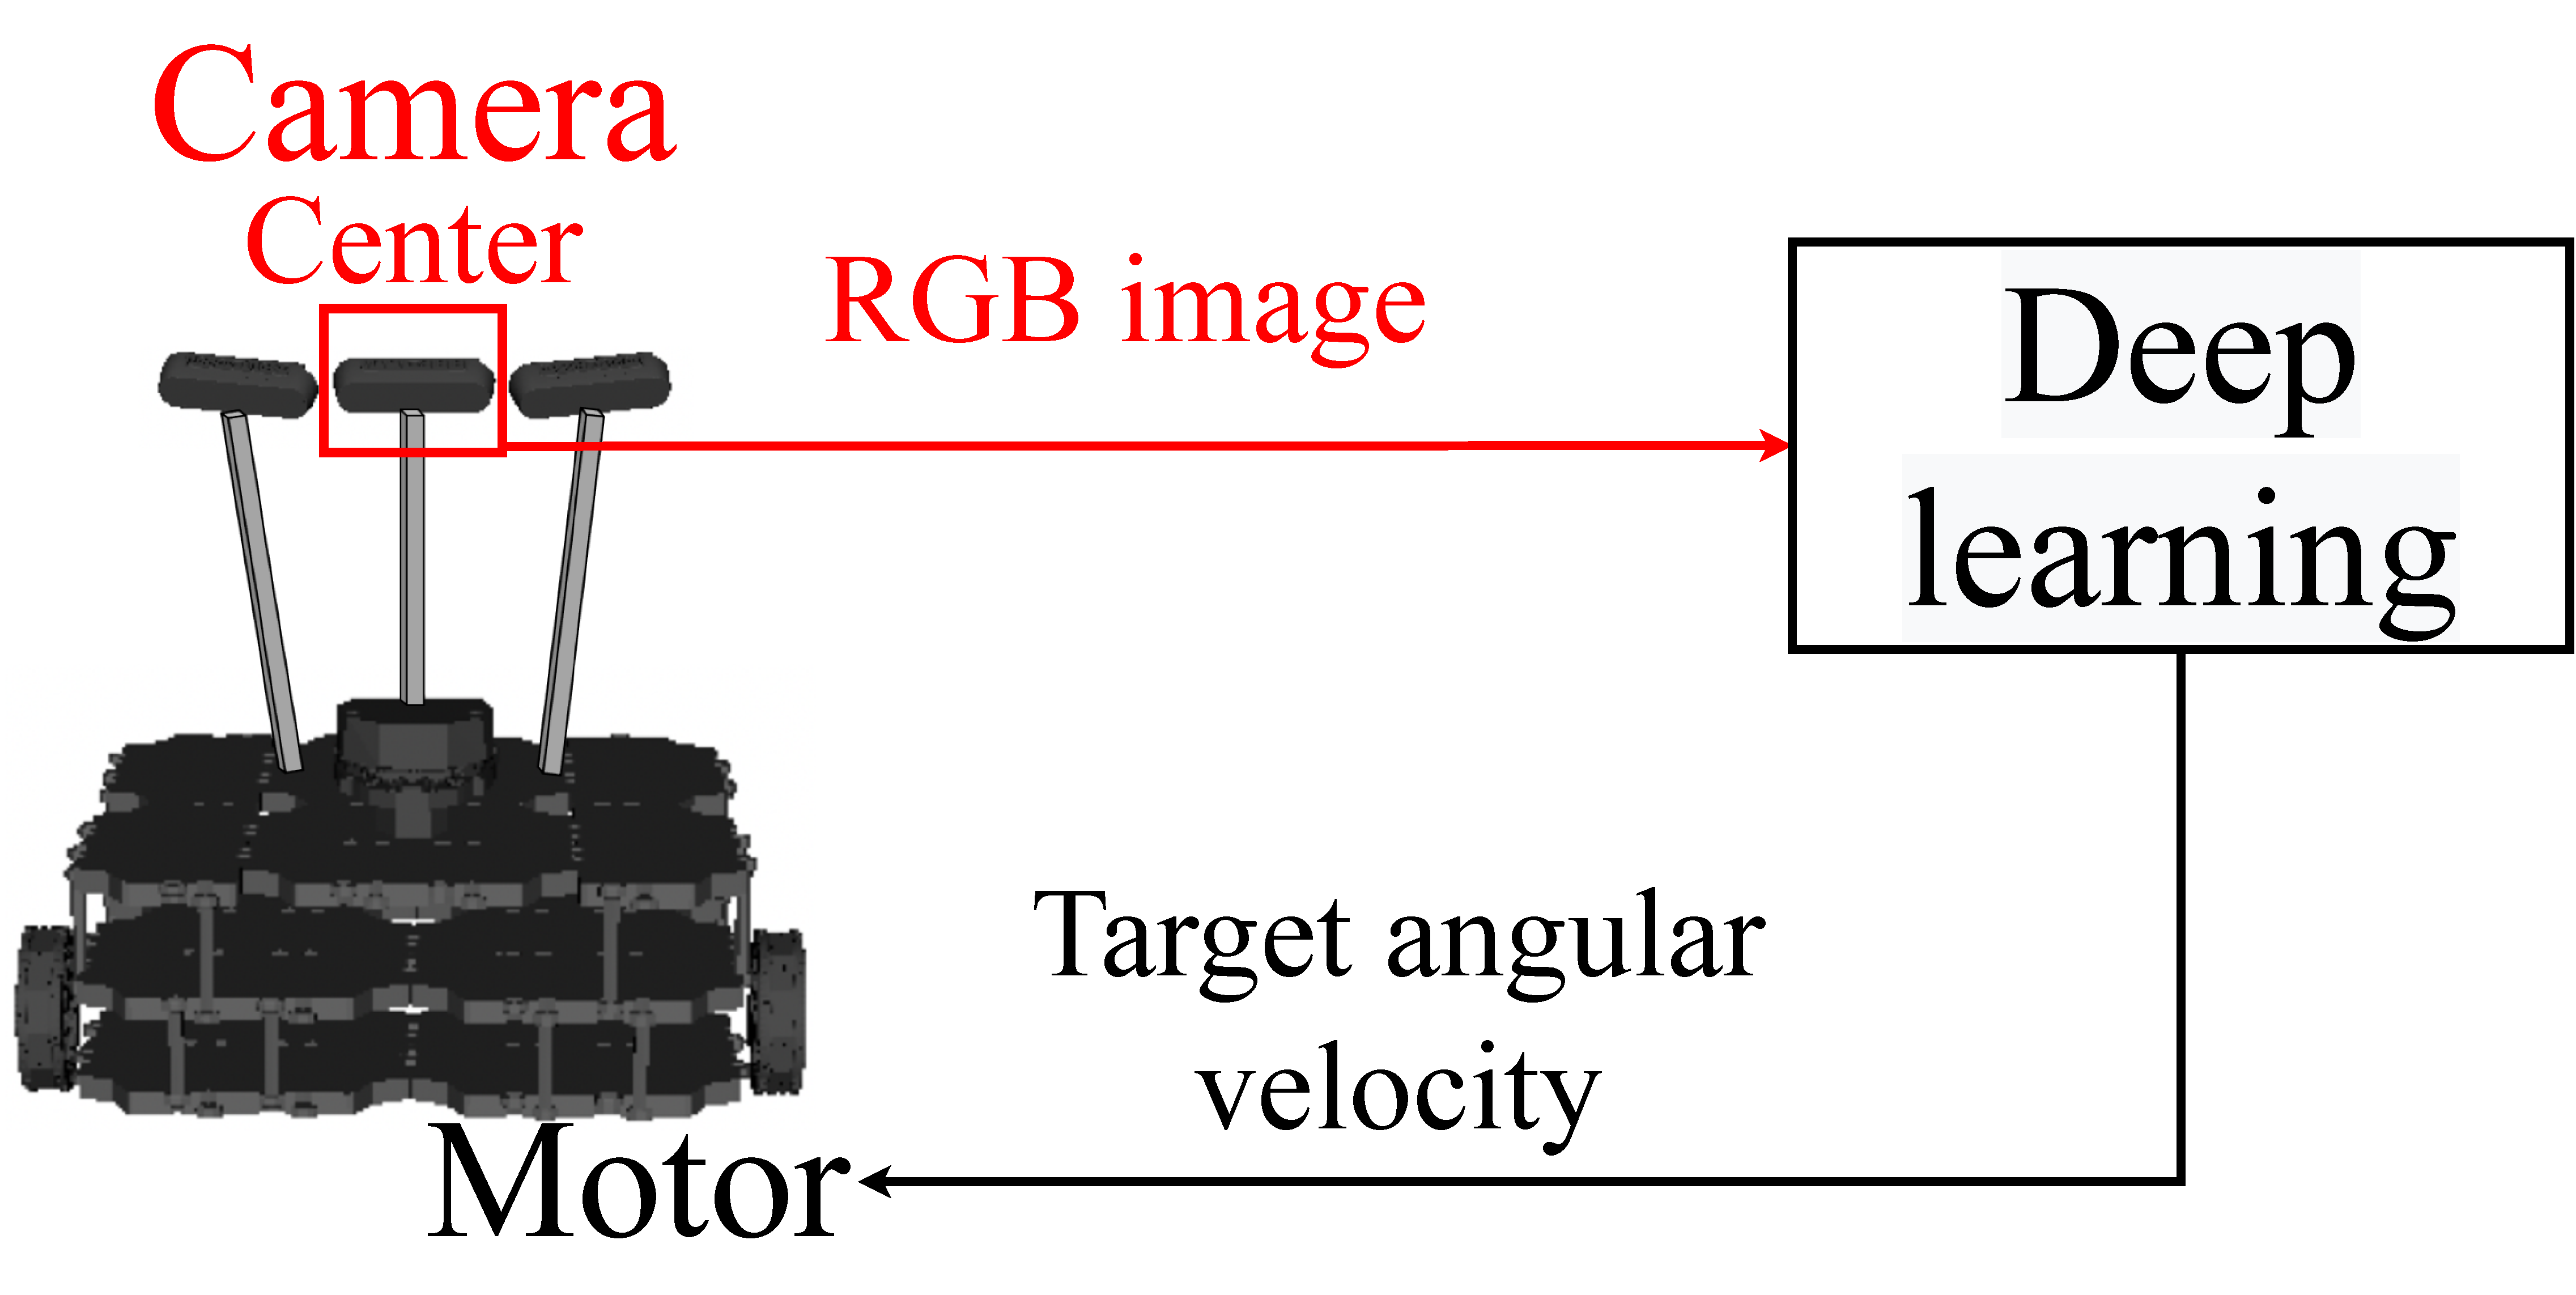
\includegraphics[width = 10cm]{./figs/okada_method_test.pdf}
    \caption{Test phase of conventional method}
    \label{fig::okada_method_test}
\end{figure}
% \include{purpose}MK
%提案手法
\chapter{提案手法}\label{chap:method}
本章では,従来手法をベースとする提案手法を
提案手法の概要,提案手法における学習フェーズ,テストフェーズと用いた目標方向について
の4節に分けて述べる.

\section{提案手法の概要}

% 1章の背景で述べた分岐路において,ルートを選択する場合に
% 入力する情報としてカメラ画像のみでは「右と左のどちらに曲がる」という判断をするための
% 情報が不足していると考えられる.
従来手法で用いたデータセットと学習器の入力へ,
「直進」「左折」などの目標方向を追加することで,
学習器の出力による走行において,経路を選択する機能の追加を行った.
なお,追加した要素以外は従来手法と同様である.
% 本研究で対象とするロボットの構造,搭載するセンサを\ref{fig::turtlebot3_gazo}とし,

% 提案手法の概要をFig.\ref{fig::method_abs}

% \begin{figure}[H]
%     \centering
%     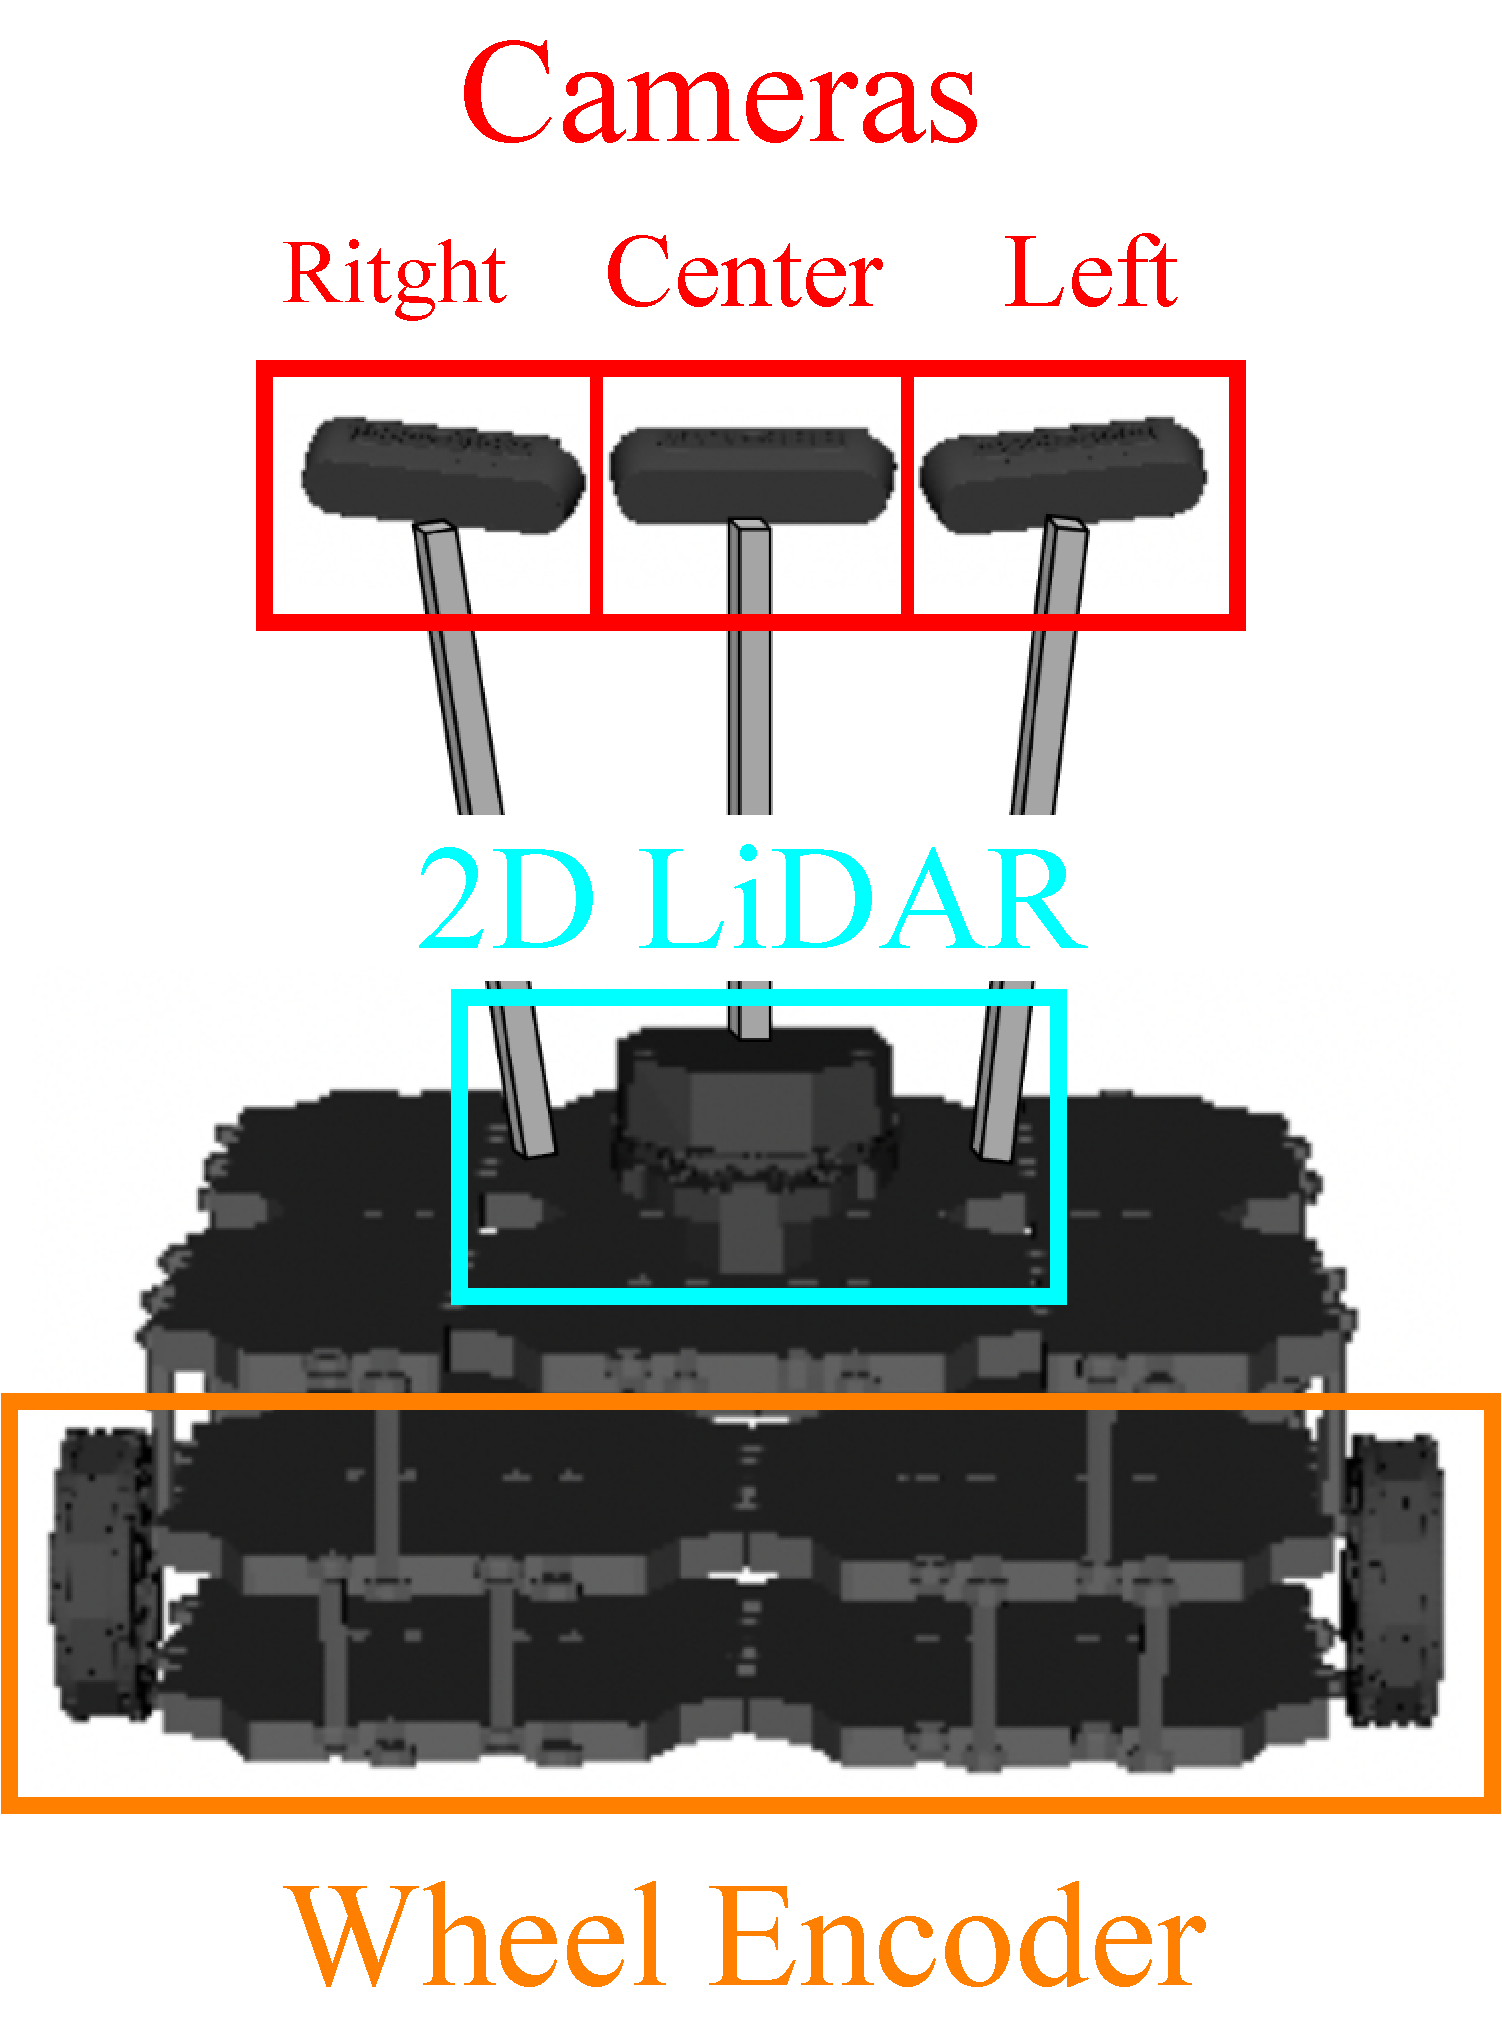
\includegraphics[width = 4cm]{./figs/turtlebot3_kame.pdf}
%     \caption{turtlebot3 waffle}
%     \label{fig::turtlebot3_gazo}
% \end{figure}

% \begin{figure}[H]
%     \begin{tabular}{c}
%       \begin{minipage}[t]{0.5\hsize}
%         \centering
%         % \vspace{-1.0zh}
%         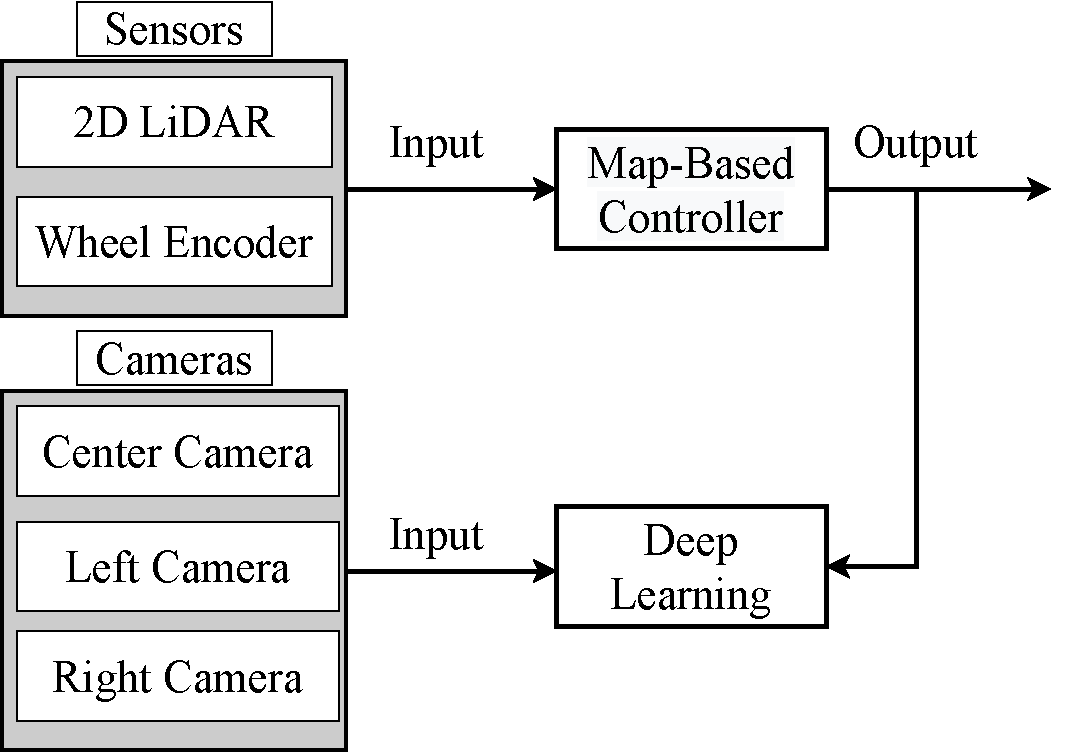
\includegraphics[keepaspectratio, scale=0.35]{./figs/system_abs.pdf}
%         \subcaption{Learning phase}
%         \label{fig::learning_abs}
%       \end{minipage}
%       \begin{minipage}[t]{0.5\hsize}
%         \centering
        
%         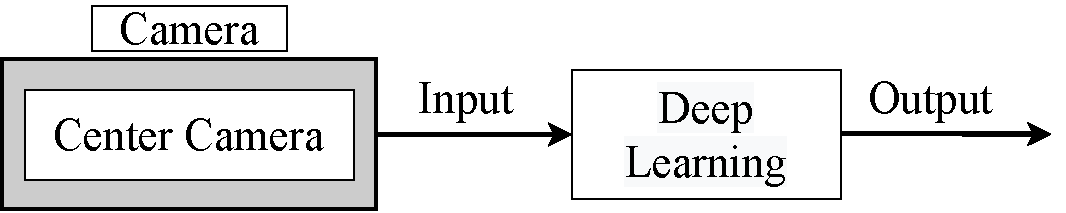
\includegraphics[keepaspectratio, scale=0.35]{./figs/system_test_abs.pdf}
%         \subcaption{Test phase}
%         \label{fig::test_abs}
%       \end{minipage}
%       \vspace{2.0zh}
%     \end{tabular}
%      \caption{Concept of the proposed method}
%      \label{fig::method_abs}
%   \end{figure} 


    
    % \begin{table}[h]
    %   \centering
    %   \caption{Target Direction list}
    %   \begin{tabular}{ccccll}
    %   \cline{1-5}
    %   \multicolumn{1}{|c|}{Target Direction} & \multicolumn{1}{c|}{continue}&\multicolumn{1}{c|}{go straight}          & \multicolumn{1}{c|}{turn left}          & \multicolumn{1}{c|}{turn right}          &  \\ \cline{1-5}
    %   \multicolumn{1}{|c|}{Data}  &\multicolumn{1}{c|}{{[}100, 0, 0, 0{]}}& \multicolumn{1}{c|}{{[}0, 100, 0, 0{]}} & \multicolumn{1}{c|}{{[}0,0,100, 0{]}} & \multicolumn{1}{l|}{{[}0, 0, 0, 100{]}} &  \\ \cline{1-5}
    %                              &                                  &                                  &                                  &  \\
    %                              &                                  &                                  &                                  &  \\
    %   \multicolumn{1}{l}{}       &                                  &                                  &                                  & 
    %   \end{tabular}
    %   \vspace{-3.0zh}
    %   \label{tb:command_4}
    %   \end{table}

\newpage
\section{学習フェーズ}
\label{lerning}
提案手法で用いる学習フェーズをFig. \ref{fig::learningsystem}に示す.
経路追従行動を行う地図べースの制御器へ目標方向の生成機能と,データセットへ目標方向の追加を行った.
提案手法では,Fig. \ref{fig::learning_abs}に示すように
LiDARとオドメトリを入力とする地図べースの制御器による経路追従行動を,
カメラ画像と目標方向を用いて模倣学習する.
  \begin{figure}[h]
    \centering
    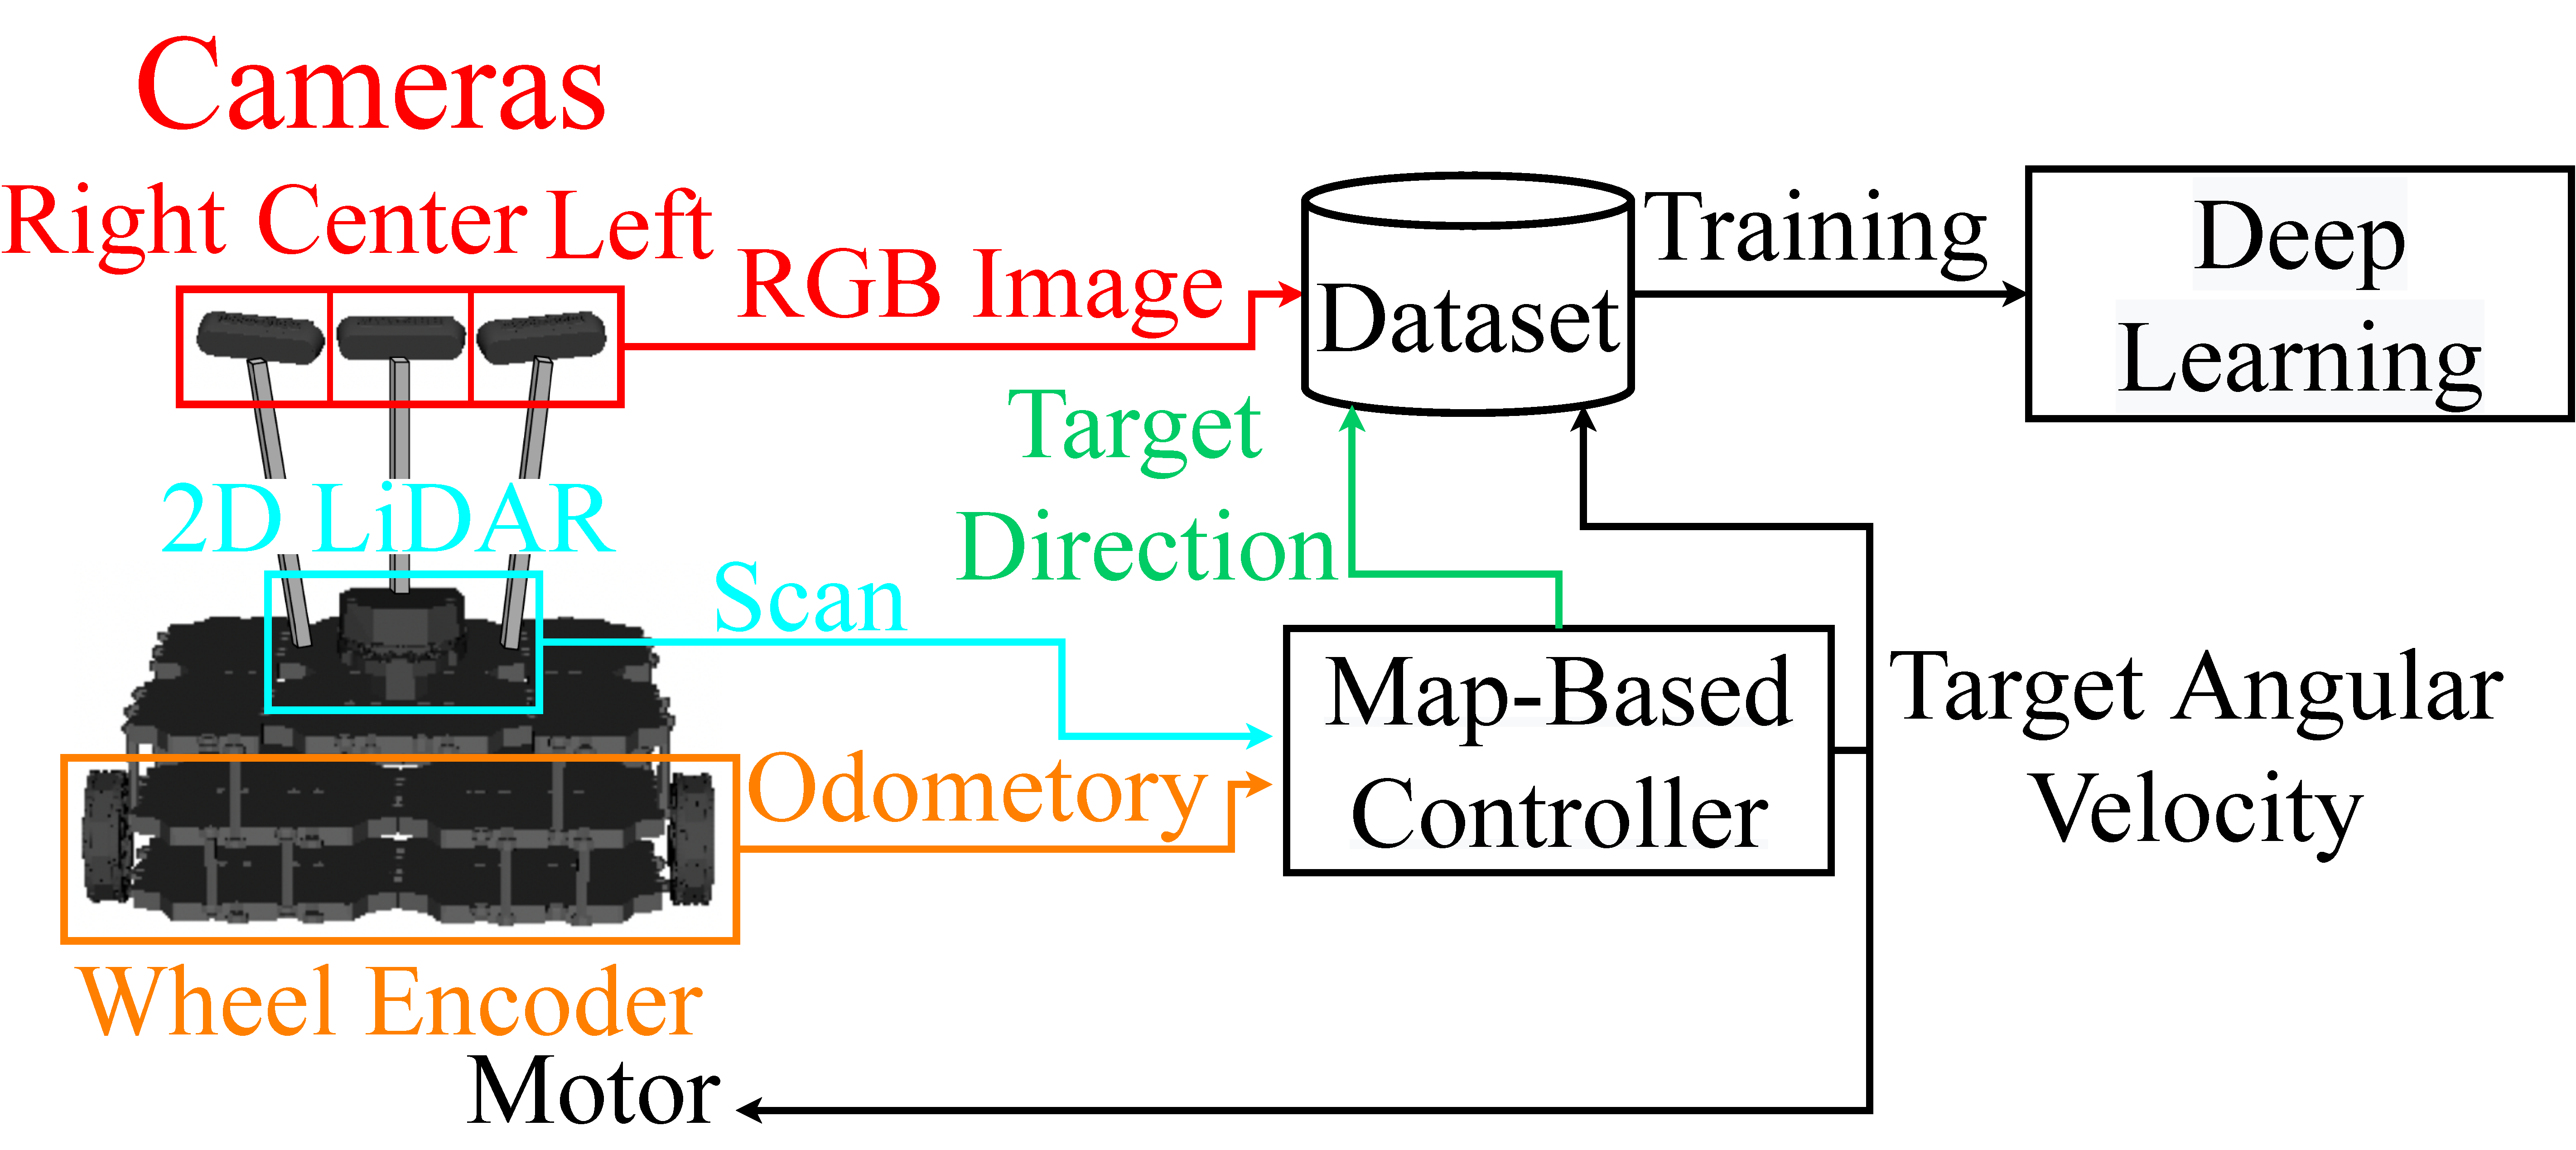
\includegraphics[width = 12cm]{./figs/system_learning.pdf}
    \caption{Learning phase of proposed method}
    \label{fig::learningsystem}
\end{figure}
\begin{figure}[h]
  \centering
  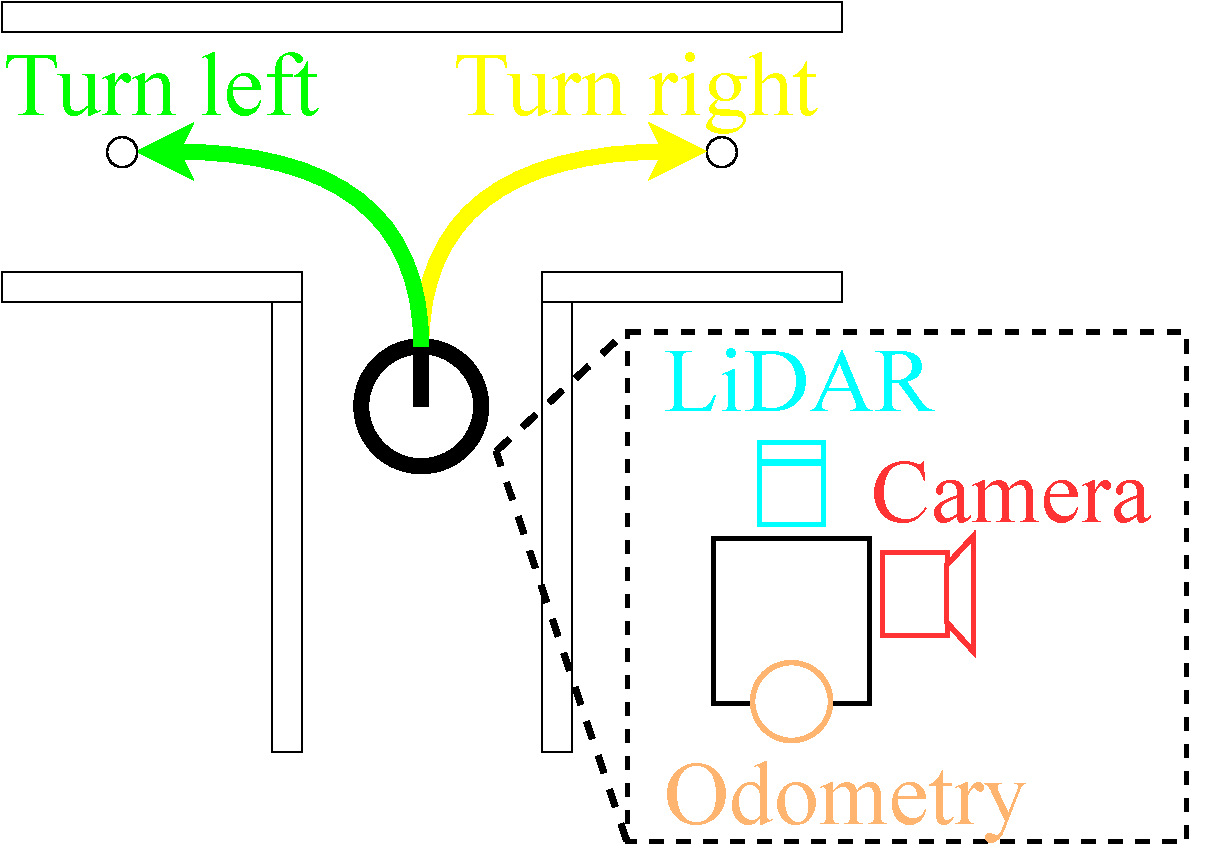
\includegraphics[width = 9.5cm]{./figs/ler_abs.pdf}
  \caption{Overview learning phase}
  \label{fig::learning_abs}
\end{figure}
\newpage
\section{テストフェーズ}
\label{test}
提案手法におけるテストフェーズではFig. \ref{fig::testsystem}で示すように,
学習器の入力へ目標方向を加えた.
Fig. \ref{fig::test_abs}に動作の様子を示す.
カメラ画像と目標方向を用いた学習器の出力による走行において,目標方向によって経路の選択を行う.
% 地図ベースの制御器の出力による動作から,中央のカメラ画像と目標方向を入力とした
% 学習器の出力による動作へ切り替えて走行を行う.
% テスト時の目標方向の生成(方向の指示)はJoy\_stickコントローラのボタンを用いて行う.
% また,目標方向は学習フェーズと同じ形式,データを用いる.
% テストフェーズにおける手順を下記に示す.
% \begin{enumerate}
%     \item 機体に取り付けた中央のカメラからRGB画像,Joy\_stickコントローラより目標方向のデータを取得
%     \item 取得したデータ(カメラ画像,目標方向)を学習器へ入力
%     \item 学習器の出力である角速度をモータへ与える
%   \end{enumerate}

\begin{figure}[h]
    \centering
    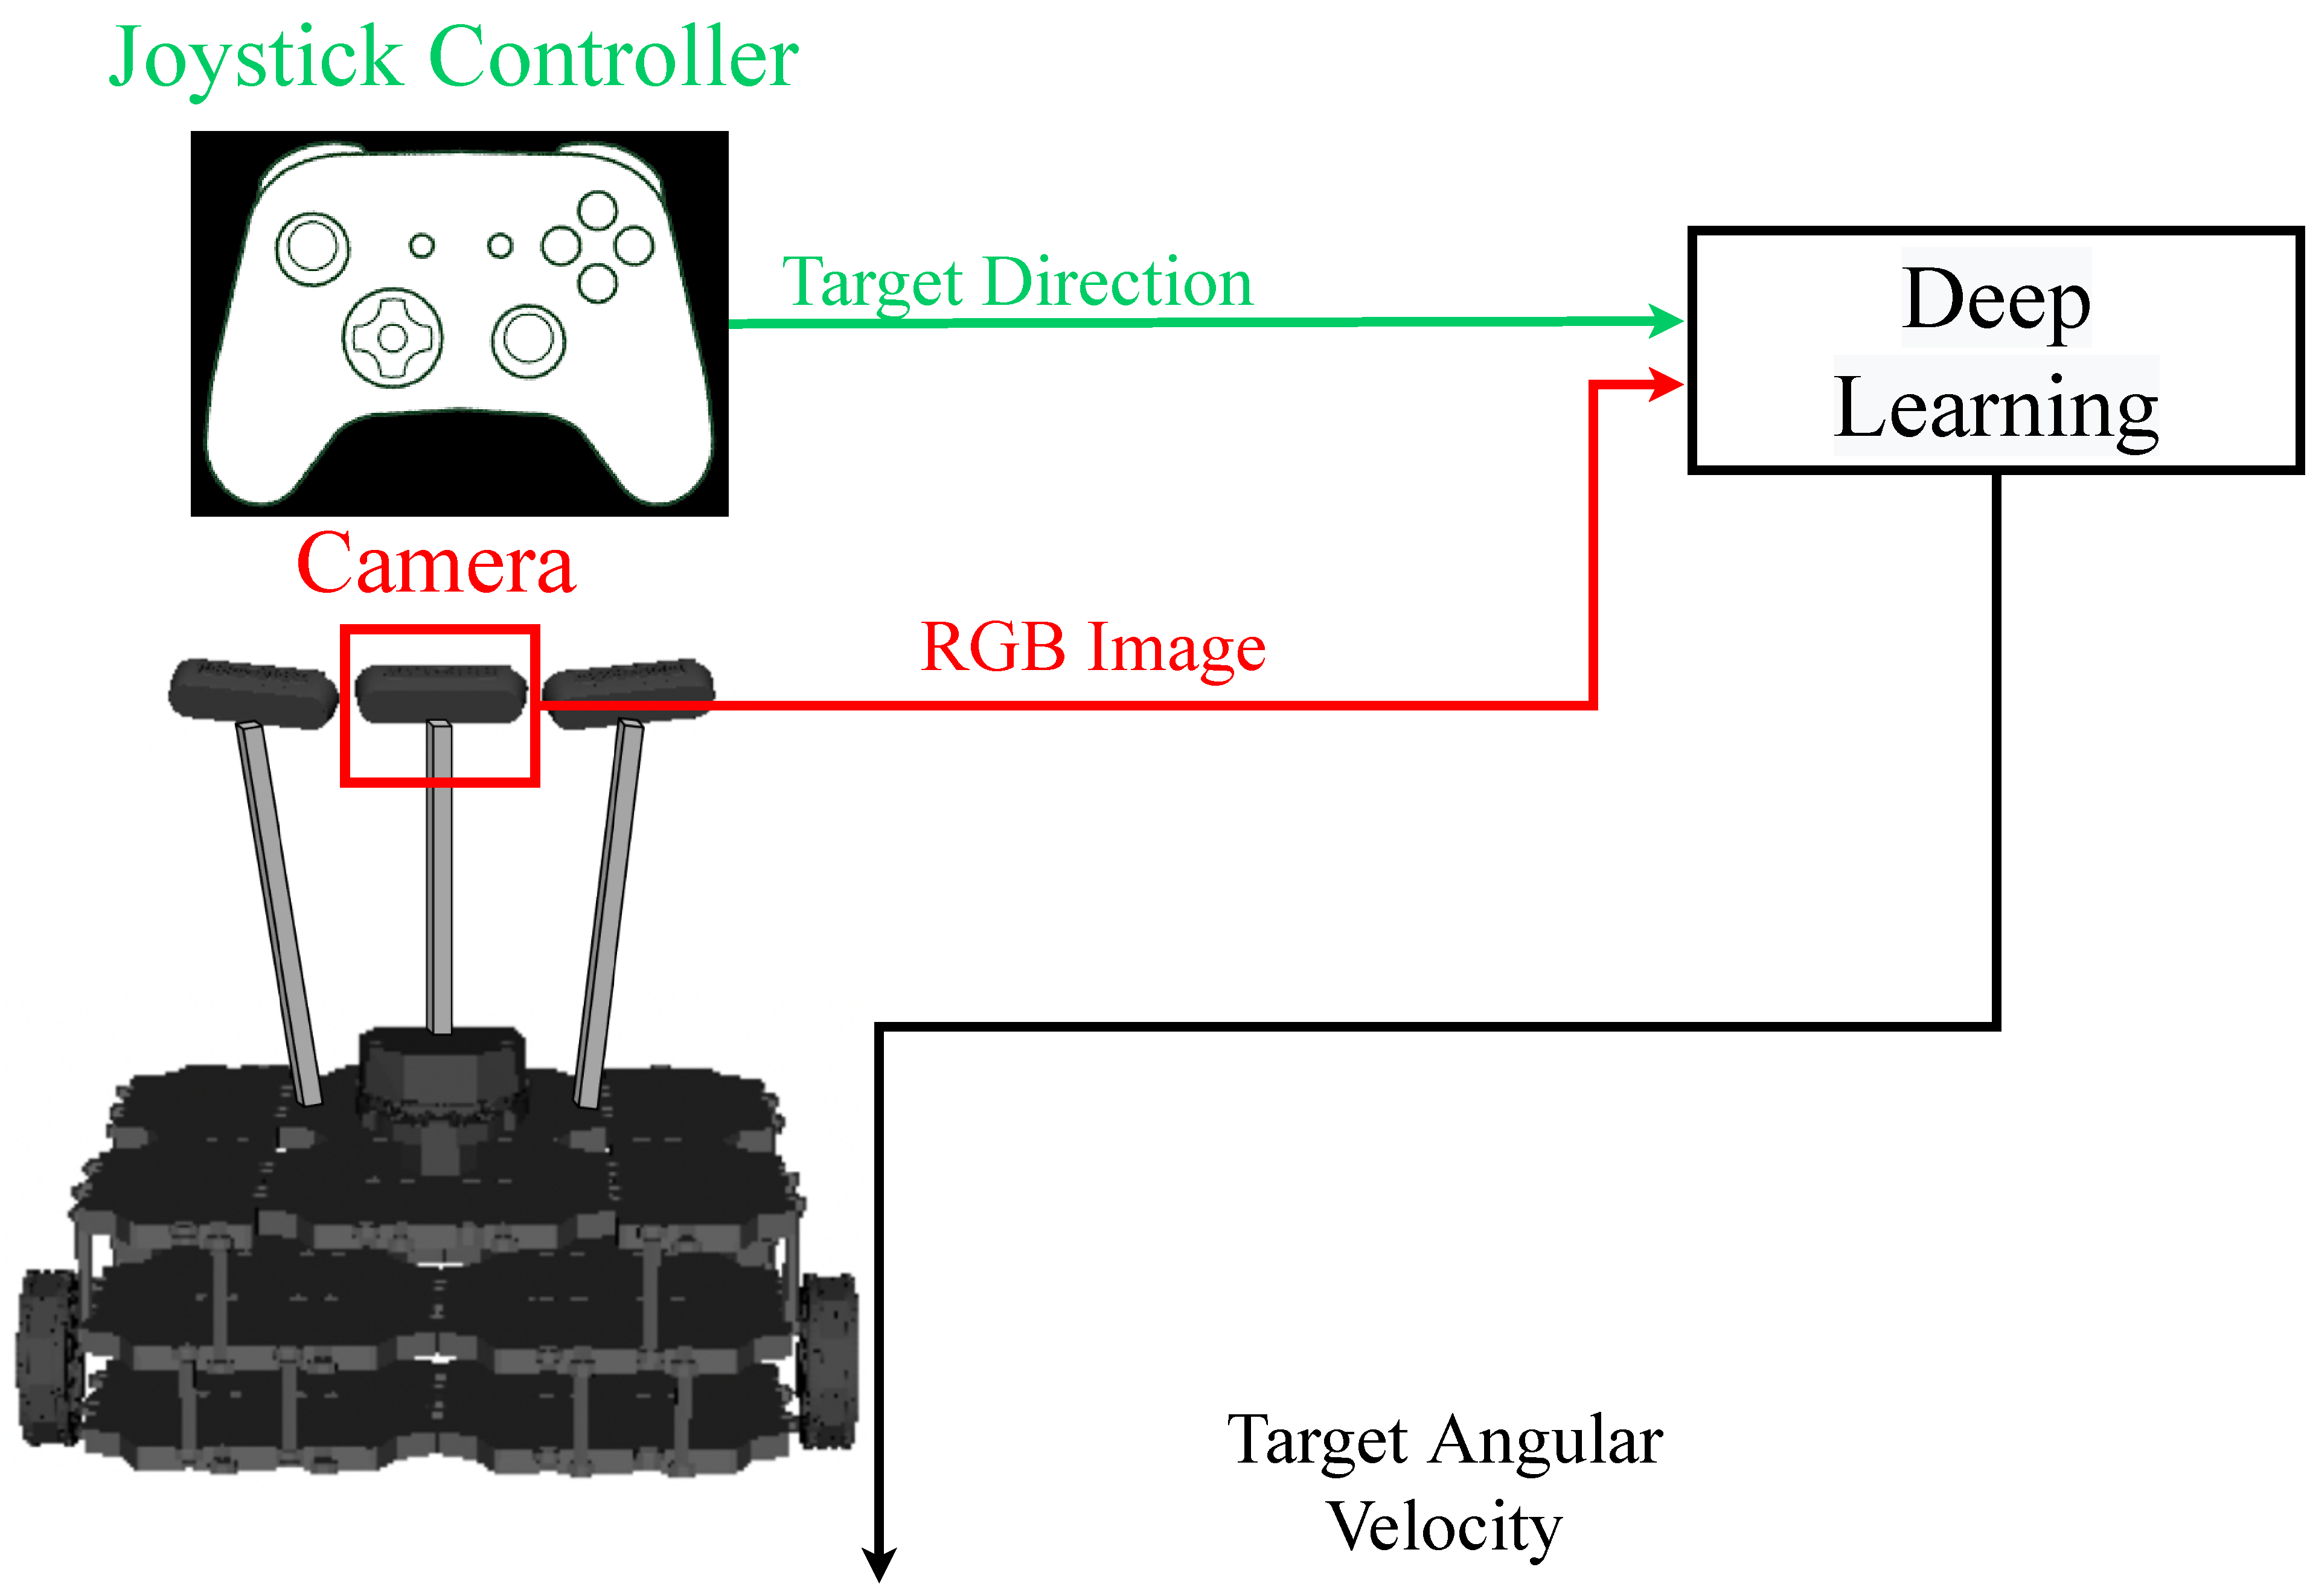
\includegraphics[width = 9cm]{./figs/system_test.pdf}
    \caption{Test phase of proposed method}
    \label{fig::testsystem}
\end{figure}
\begin{figure}[h]
  \centering
  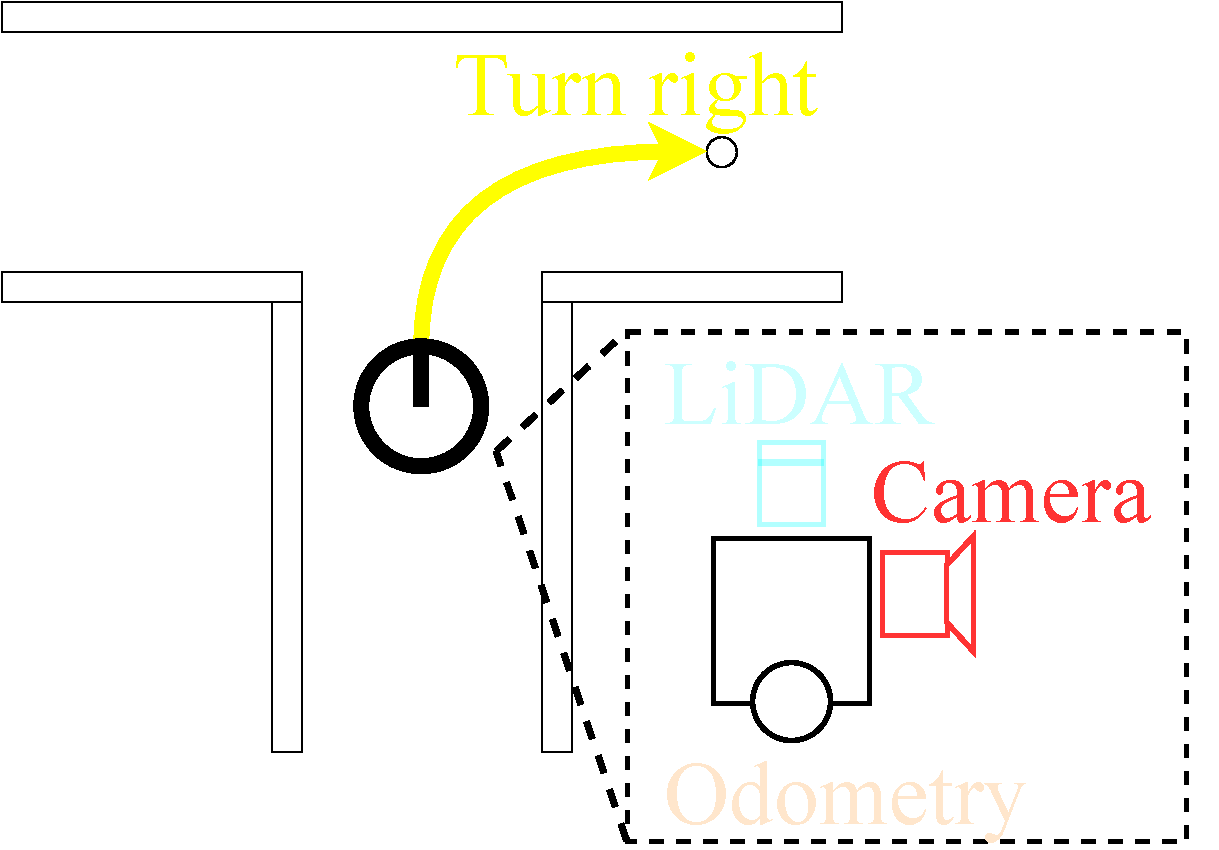
\includegraphics[width = 9cm]{./figs/test_abs.pdf}
  \caption{Overview test phase}
  \label{fig::test_abs}
\end{figure}

\newpage
\section{目標方向}
本研究で用いた目標方向と,そのデータ形式である目標方向指令について述べる.
目標方向をFig.\ref{fig::cmd_4}に示す.
経路を「道なり」に走行(Continue)
分岐路において「直進(Go straight)「左折(Turn left)」「右折(Turn right)」の4つとする,
\begin{figure}[h]
  \centering
  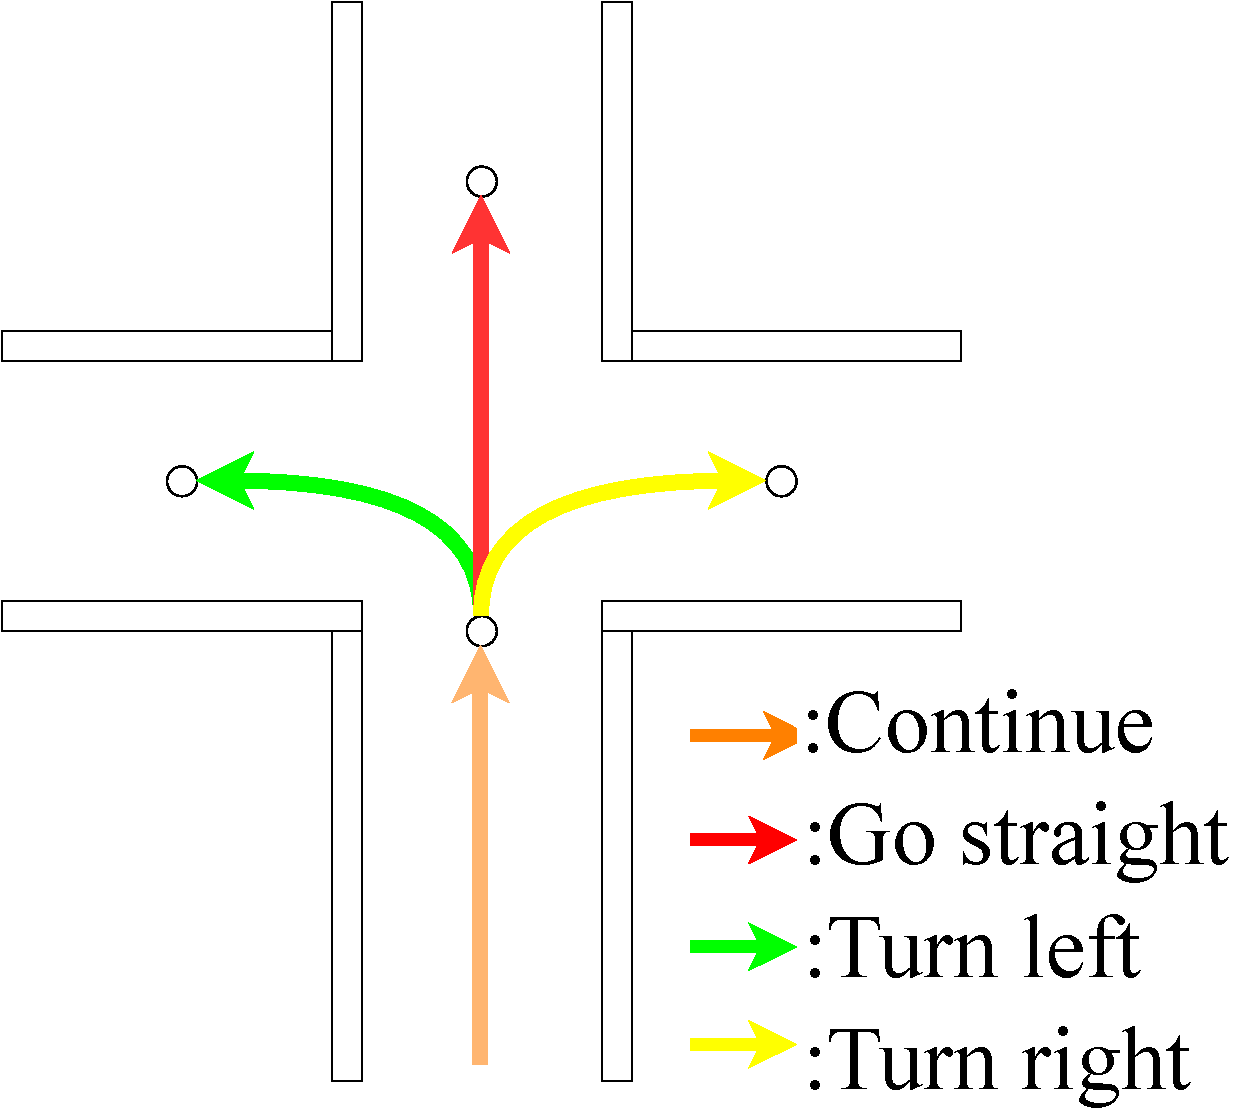
\includegraphics[width = 9.5cm]{./figs/cmd_4.pdf}
  \caption{Target direction}
  \label{fig::cmd_4}
\end{figure}

学習器には,上記の4つの目標方向を,要素数4,次元数1のint型の
配列(One-Hot ベクトル)で表現した”目標方向指令”を入力する.
目標方向指令のデータ形式をTable \ref{tb:command_4}に示す.
  %   \begin{table}[h]
  %     \caption{Target direction and data}
  %     \label{tb:command_4}
  %     \begin{center}
  %         \vskip 0.5zh
  %         \begin{tabular}{|c|c|}
  %             \hline
  %             Target direction & Data\\ \hline
  %             Continue & $[100, 0, 0, 0]$ \\ \hline
  %             Go straight & $[0, 100, 0, 0]$ \\ \hline
  %             Turn left& $[0, 0, 100, 0]$ \\ \hline
  %             Turn right & $[0, 0, 0, 100]$ \\ \hline
  %         \end{tabular}
  %     \end{center}
  % \end{table}

 \begin{table}[h]
      \centering
      \caption{Target direction list}
      \begin{tabular}{ccccll}
      \cline{1-5}
      \multicolumn{1}{|c|}{Target Direction} & \multicolumn{1}{c|}{Continue}&\multicolumn{1}{c|}{Go straight}          & \multicolumn{1}{c|}{Turn left}          & \multicolumn{1}{c|}{Turn right}          &  \\ \cline{1-5}
      \multicolumn{1}{|c|}{Data}  &\multicolumn{1}{c|}{{[}100, 0, 0, 0{]}}& \multicolumn{1}{c|}{{[}0, 100, 0, 0{]}} & \multicolumn{1}{c|}{{[}0, 0, 100, 0{]}} & \multicolumn{1}{l|}{{[}0, 0, 0, 100{]}} &  \\ \cline{1-5}
                                 &                                  &                                  &                                  &  \\
                                 &                                  &                                  &                                  &  \\
      \multicolumn{1}{l}{}       &                                  &                                  &                                  & 
      \end{tabular}
      \vspace{-3.0zh}
      \label{tb:command_4}
      \end{table}
\newpage
\section{ネットワーク構造}
\label{net}
提案手法で用いた学習器のネットワークをFig. \ref{fig::methodnetwork}に示す.
また,ハイパーパラメータについてTable \ref{tb::param}に示す.
64×48のRGB画像を入力とする入力層1,畳込み層3,全結合層2層を持つ6層のCNNと,CNNの出力と目標方向指令を入力する入力層1,
全結合層2.出力層1の全10層の構造になっている.
出力はヨー方向の角速度である.

\begin{figure}[h]
    \centering
    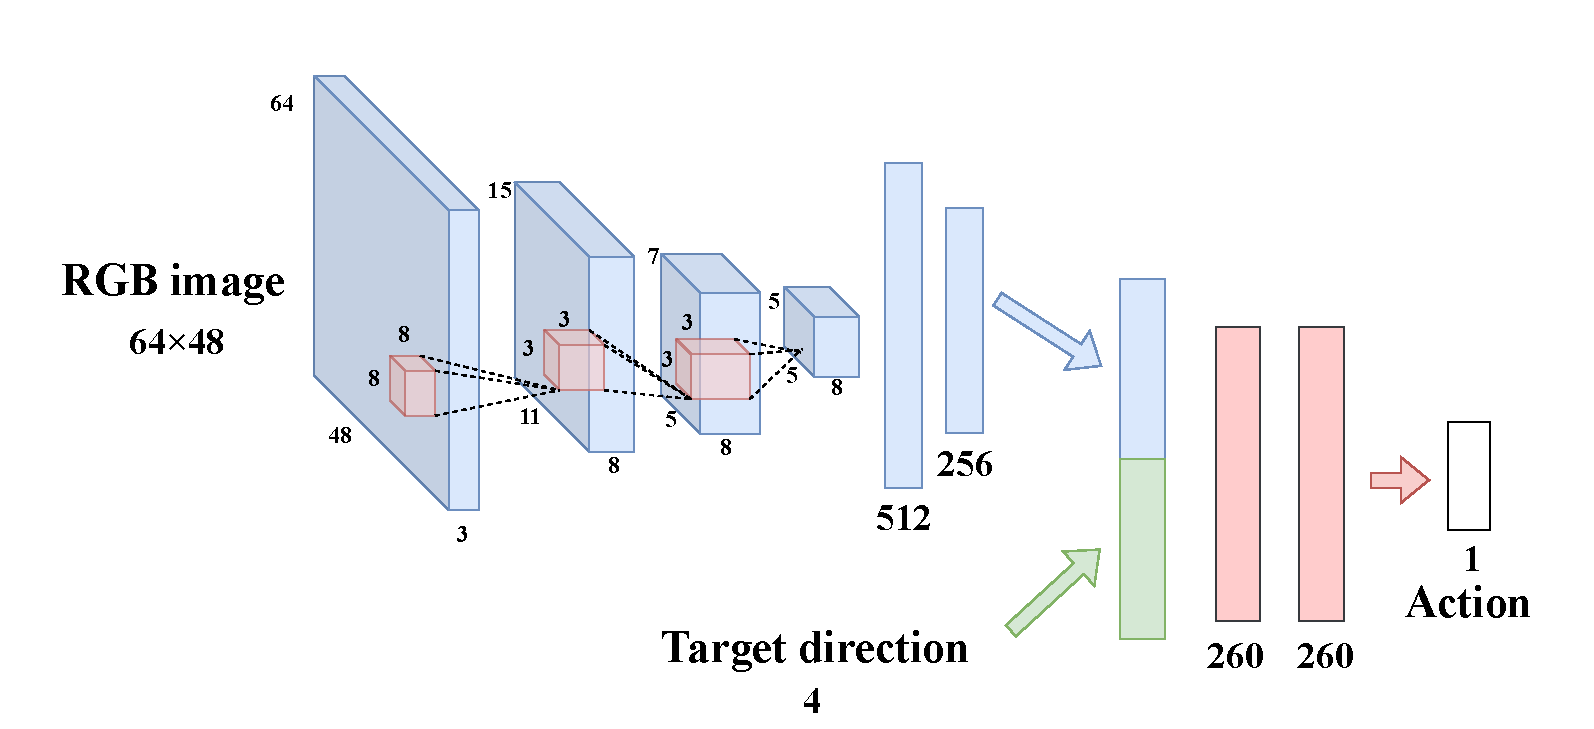
\includegraphics[width = 13cm]{./figs/method_network.pdf}
    \caption{Method network}
    \label{fig::methodnetwork}
\end{figure}
% \vspace{-1.0zh}
\begin{table}[htb]
    \centering
    \caption{Parameters of deep learning}
    \begin{tabular}{|c|c|c|c|}
    \hline
    Input data    & Image (64x48 pixels, RGB channels) , Target direction                                             \\ \hline
    Optimizer     & Adam ($alpha = 0.001, beta1 = 0.9, beta2 = 0.999, eps = 1e^{-1}$ )  \\ \hline
    Loss function & Softmax-cross-entropy                                                            \\ \hline
    Output data   & Angular velocity                                              \\ \hline
    \end{tabular}
    \label{tb::param}
    \end{table}






%実験
\chapter{実験}
\section{実験目的}
シュミレータ上で,環境を変えて実験を行い,提案手法の有効性の検証を行う.
\section{実験環境}
実験はシミュレータ上で行う.
シミュレータ環境としてオープンソースの
3DロボットシミュレータGazebo\cite{gazebo:online}を用いる.
実験装置として,Fig. \ref{fig::turtlebot3}に示す,turtlebot3\_waffle\cite{turtlebot3:online}へカメラを
3つ追加したモデルを用いる.

\begin{figure}[H]
    \centering
    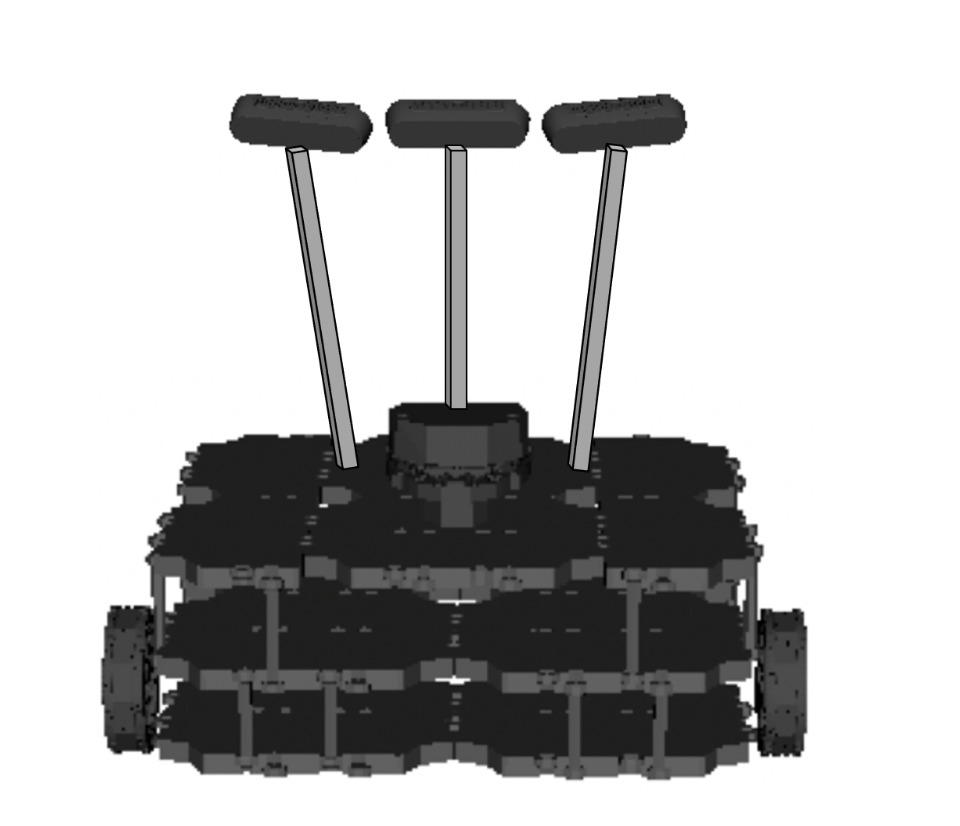
\includegraphics[width = 7cm]{./figs/3_camera.png}
    \caption{Turtlebot3 waffle with 3 cameras}
    \label{fig::turtlebot3}
\end{figure}

\section{実験方法}

実験における手順を下記に示す.
\begin{enumerate}
  \item 設定した経路を学習フェーズで走行し,学習器の訓練(経路の学習)を行う.
  \item テストフェーズへ移行,各経路を設定した回数走行する.
\end{enumerate}
なお,学習器の訓練は「訓練データ (カメラ画像, 目標方向指令) を学習器へ入力し,結果を出力」を 1step とする.
データセットの収集及び,学習器への入力は0.25[s]周期で行う.
また走行に用いる並進速度は0.2[m/s]とする.

\section{実験条件}
実験条件は
テストフェーズにおいて,
\begin{itemize}
  \item 成功:壁に衝突せず, 指定した目標地点へ到達
  \item 失敗:目標方向指令とは異なった経路を選択, または壁に衝突
\end{itemize}
とした.
\newpage
\section{実験1 (十字路を用いた実験)}
\subsection{実験目的}
十字路の単純な環境を用いて,提案手法に基づいて,追加した機能の検証を行う.
\subsection{実験環境}
Fig. \ref{fig::zyuzi}に環境,学習とテストに用いる経路と目標方向を示す.
環境は2.5m幅の十字路の環境を用いる.
この環境へ,ロボットを青で示す初期位置,姿勢で配置する.
経路は下記の手順を6000[step]学習するまで,繰り返し走行する.
なおB,C,DのTarget pointに到達次第,Startの位置へロボットの位置,姿勢を移動させる.
\begin{enumerate}
  \setlength{\parskip}{0cm} % 段落間
  \setlength{\itemsep}{0cm} % 項目間
  \item Start - A - Target point(B)
  \item Start - A - Target point(C)
  \item Start - A - Target point(D)
  \end{enumerate}

\begin{figure}[H]
    \centering
    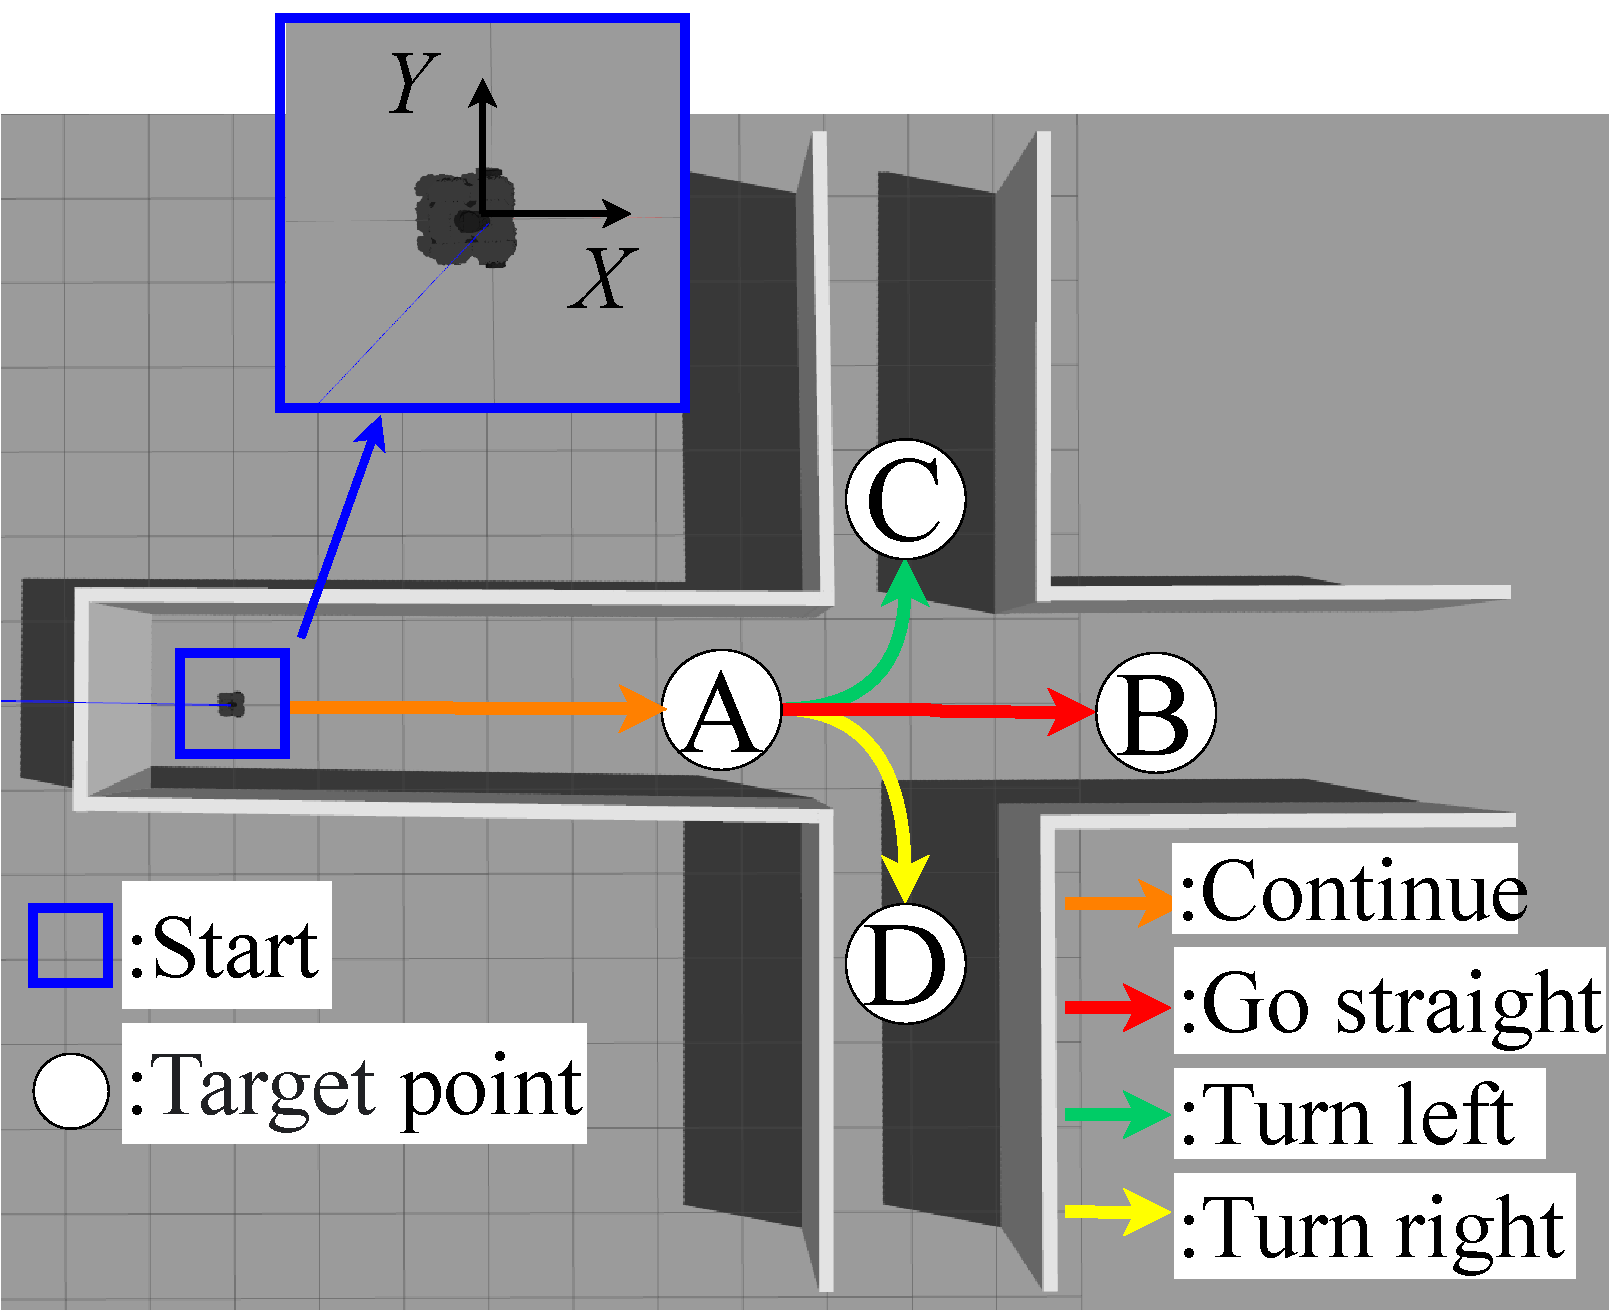
\includegraphics[width = 9.5cm]{./figs/zyuziroute.pdf}
    \caption{Experiment1 course}
    \label{fig::zyuzi}
\end{figure}

% \newpage
% \subsection{学習フェーズでの経路}
% 学習時の経路についてFig. \ref{fig::exp1route}に示す
% Fig内の緑で示す箇所が初期位置,赤で示す円が目標地点である
% 目標地点を1,2,3の順で走行し,到達後初期値点へロボットの位置,姿勢をリセットする.

% \begin{figure}[ht]
%     \centering
%     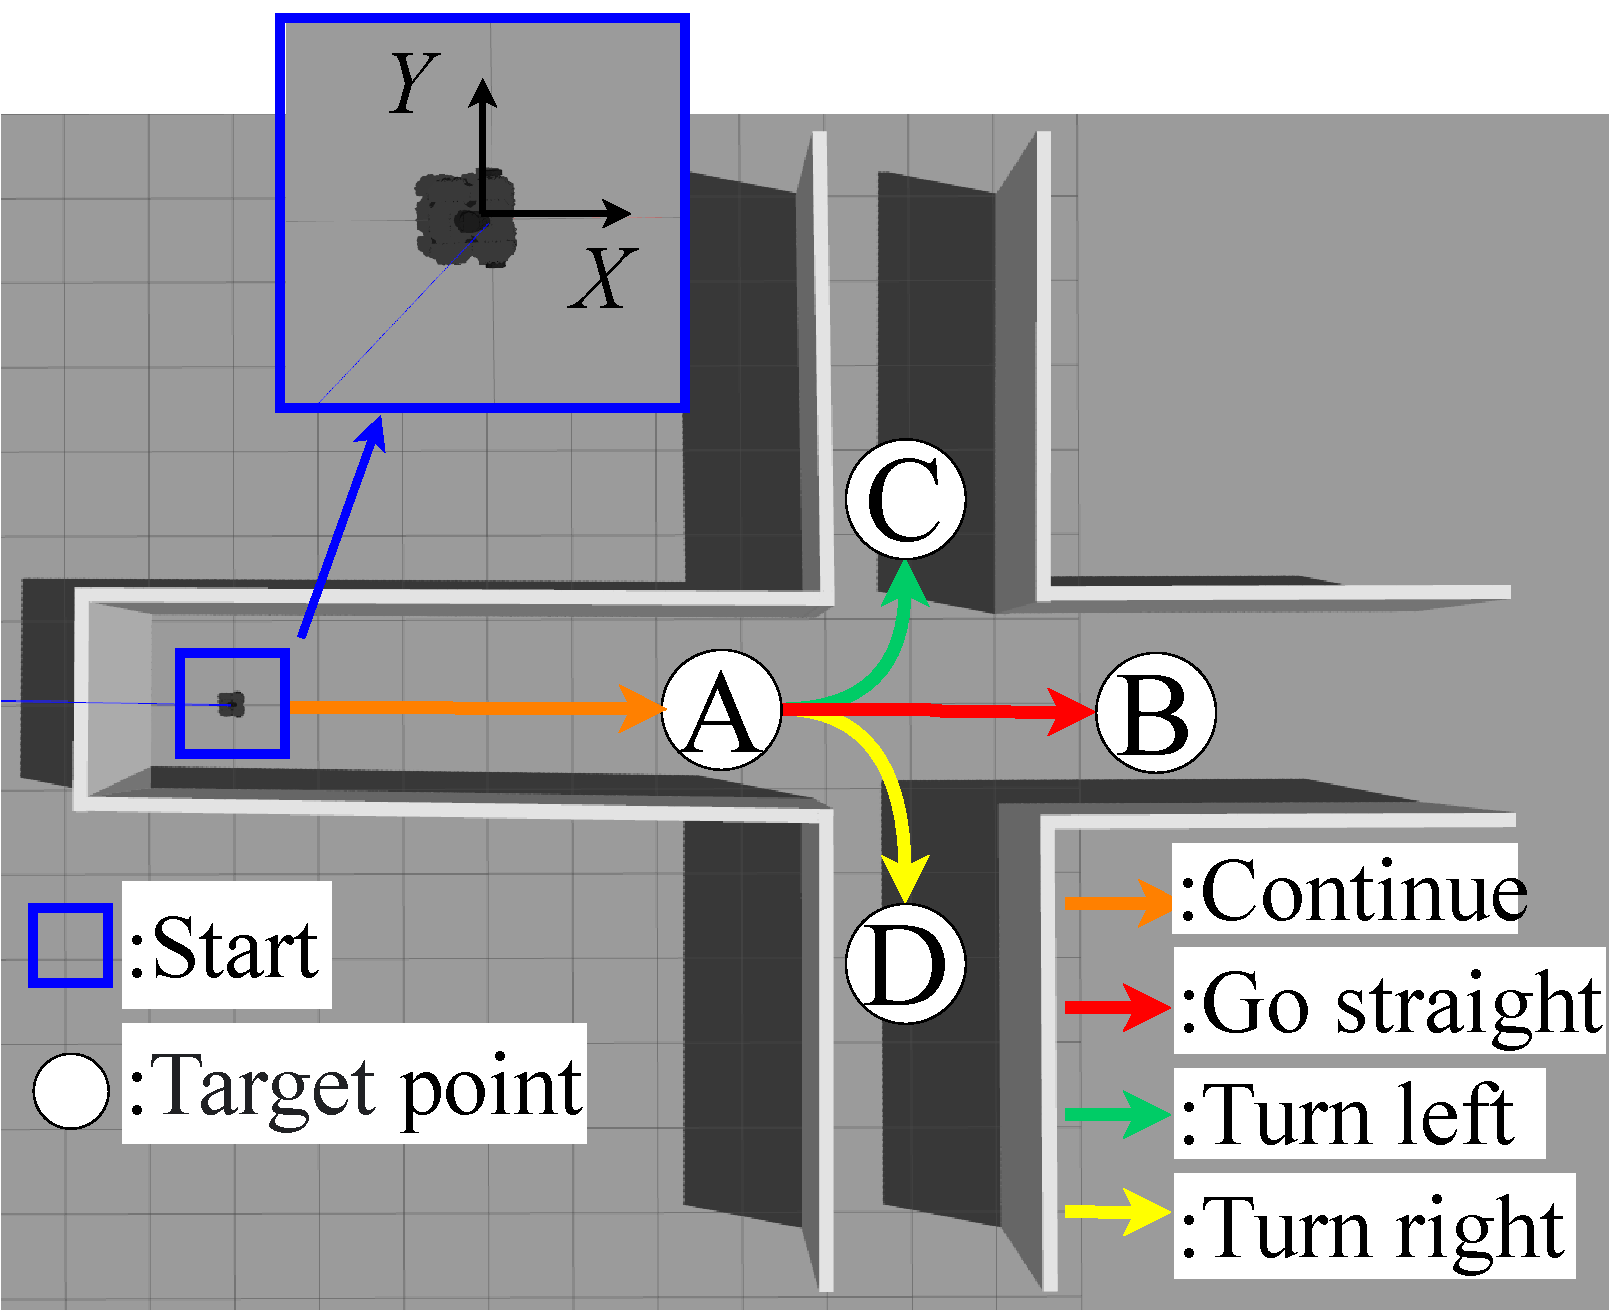
\includegraphics[width = 10cm]{./figs/zyuziroute.pdf}
%     \caption{Route of experiment 1}
%     \label{fig::exp1route}
% \end{figure}

\subsection{評価}
実験の様子をFig. \ref{fig::exp1_view}に示す.
Fig. \ref{exp1_ler_go}, \ref{exp1_ler_left}, \ref{exp1_ler_right}に示す学習フェーズでは,
赤で示した地図ベースの制御器による経路計画へ,追従して走行する様子が確認できた.
また,Fig. \ref{exp1_test_go}, \ref{exp1_test_left}, \ref{exp1_test_right}に示すテストフェーズでは,
目標方向によって,経路を選択する挙動が確認できた.
\begin{figure}[H]
  \begin{tabular}{cc}
    \begin{minipage}[t]{0.5\hsize}
      \centering
      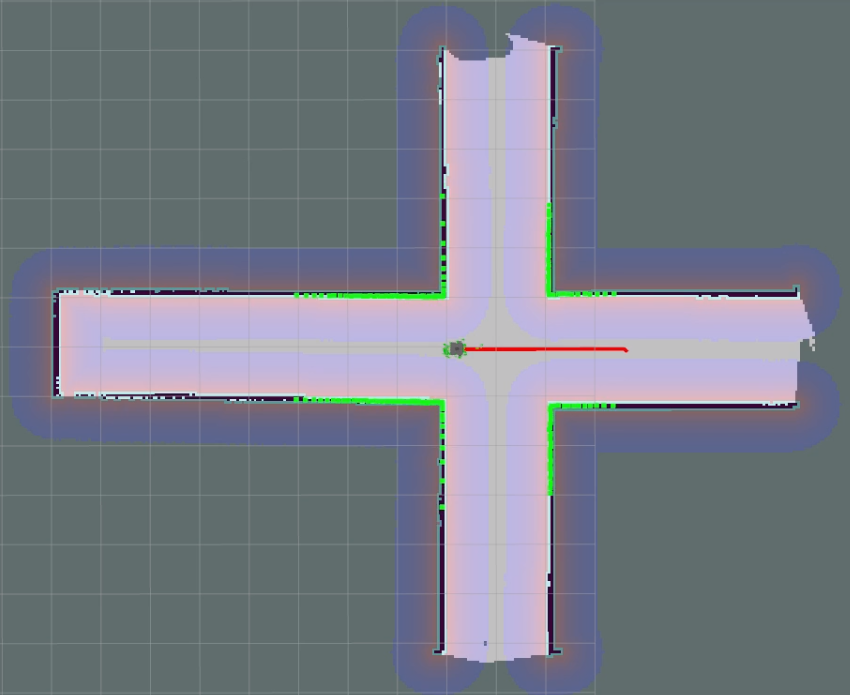
\includegraphics[width=\linewidth]{./figs/zyuzi_ler_go.png}
      \subcaption{Learning phase (target direction:go straight)}
      \label{exp1_ler_go}
    \end{minipage} 
    \begin{minipage}[t]{0.5\hsize}
      \centering
      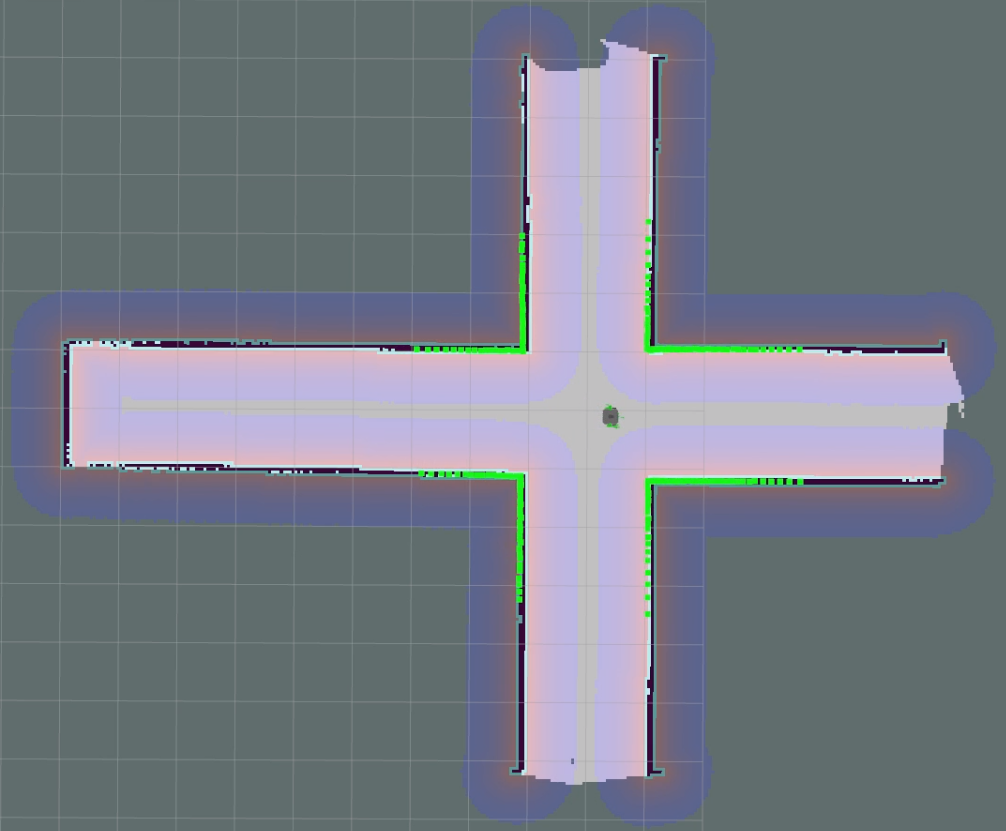
\includegraphics[width=\linewidth]{./figs/zyuzi_test_go.png}
      \subcaption{Test phase (target direction:go straight)}
      \label{exp1_test_go}
    \end{minipage} \\
    \vspace{2.0zh}
    \begin{minipage}[t]{0.5\hsize}
      \centering
      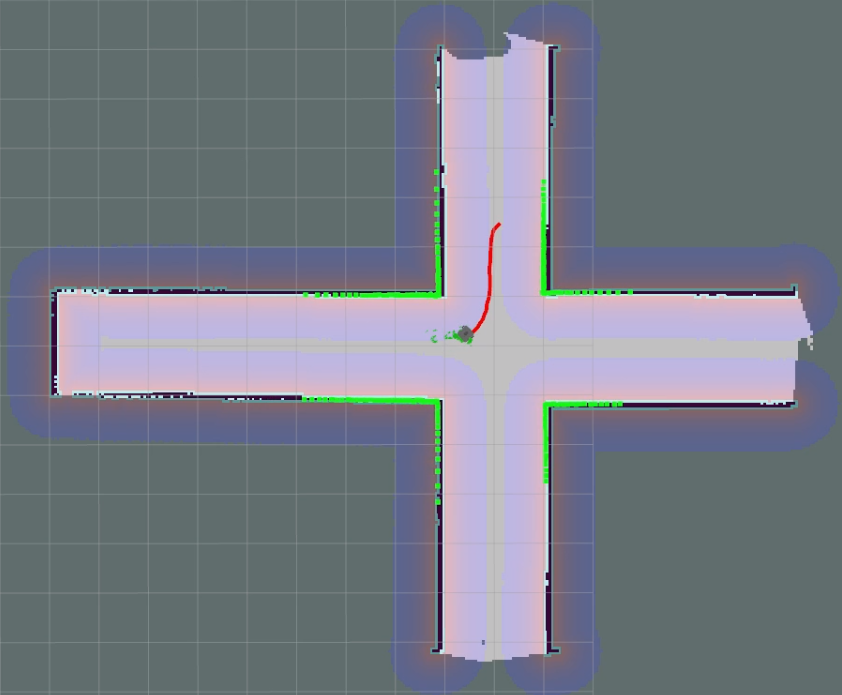
\includegraphics[width=\linewidth]{./figs/zyuzi_ler_left.png}
      \subcaption{Learning phase (target direction:turn left)}
      \label{exp1_ler_left}
    \end{minipage} 
    \begin{minipage}[t]{0.5\hsize}
      \centering
      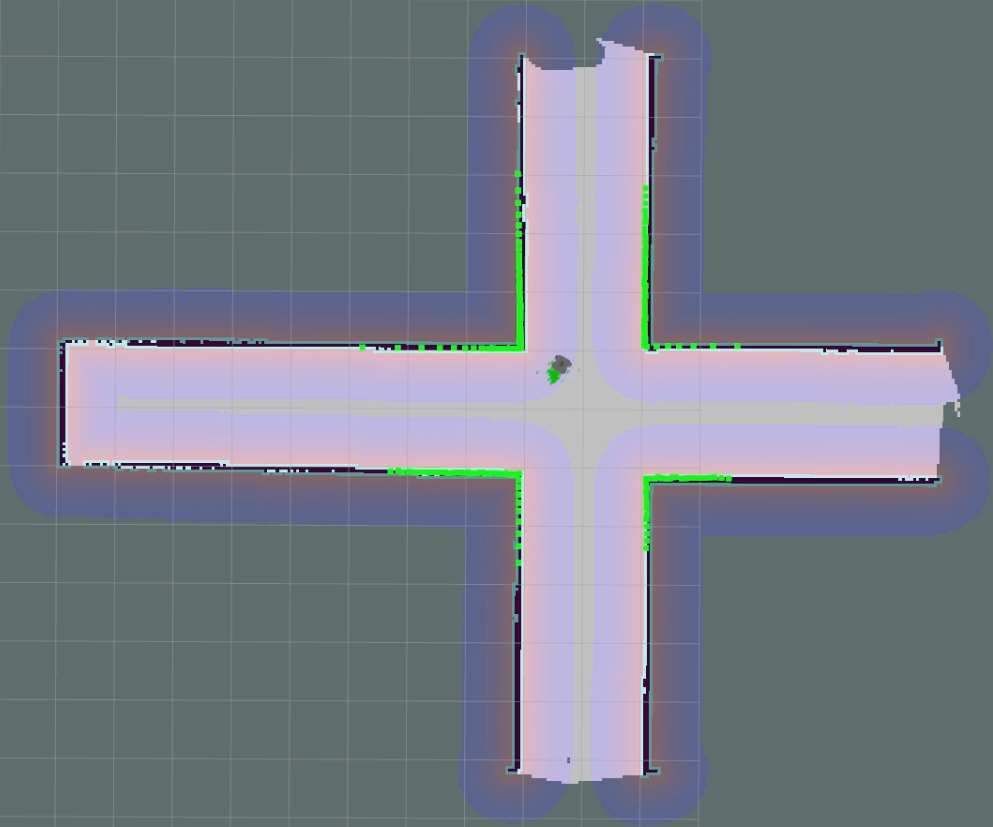
\includegraphics[width=\linewidth]{./figs/zyuzi_test_left.png}
      \subcaption{Test phase (target direction:turn left)}
      \label{exp1_test_left}
    \end{minipage}\\
    \begin{minipage}[t]{0.5\hsize}
      \centering
      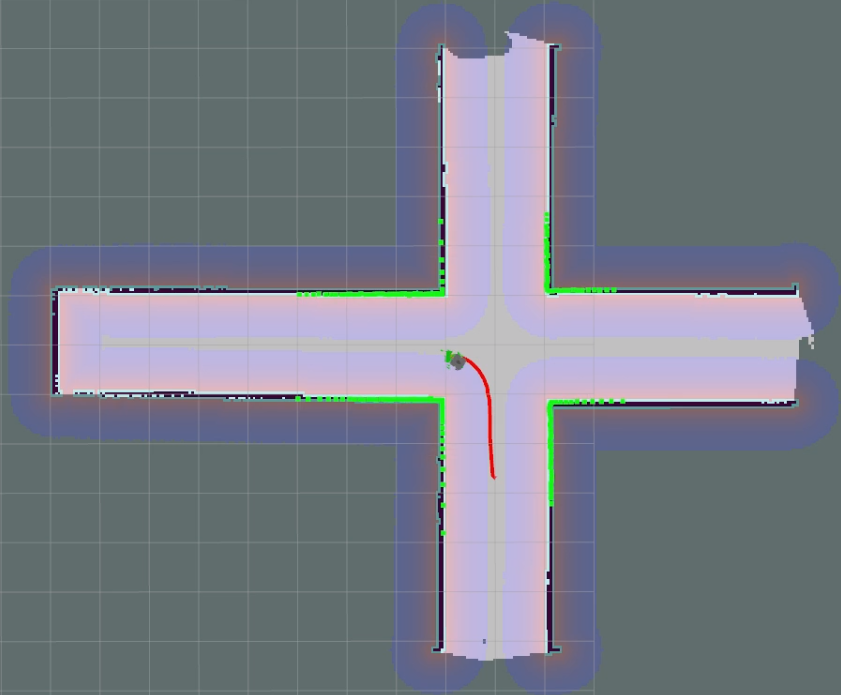
\includegraphics[width=\linewidth]{./figs/zyuzi_ler_right.png}
      \subcaption{Learning phase (target direction:turn right)}
      \label{exp1_ler_right}
    \end{minipage} 
    \begin{minipage}[t]{0.5\hsize}
      \centering
      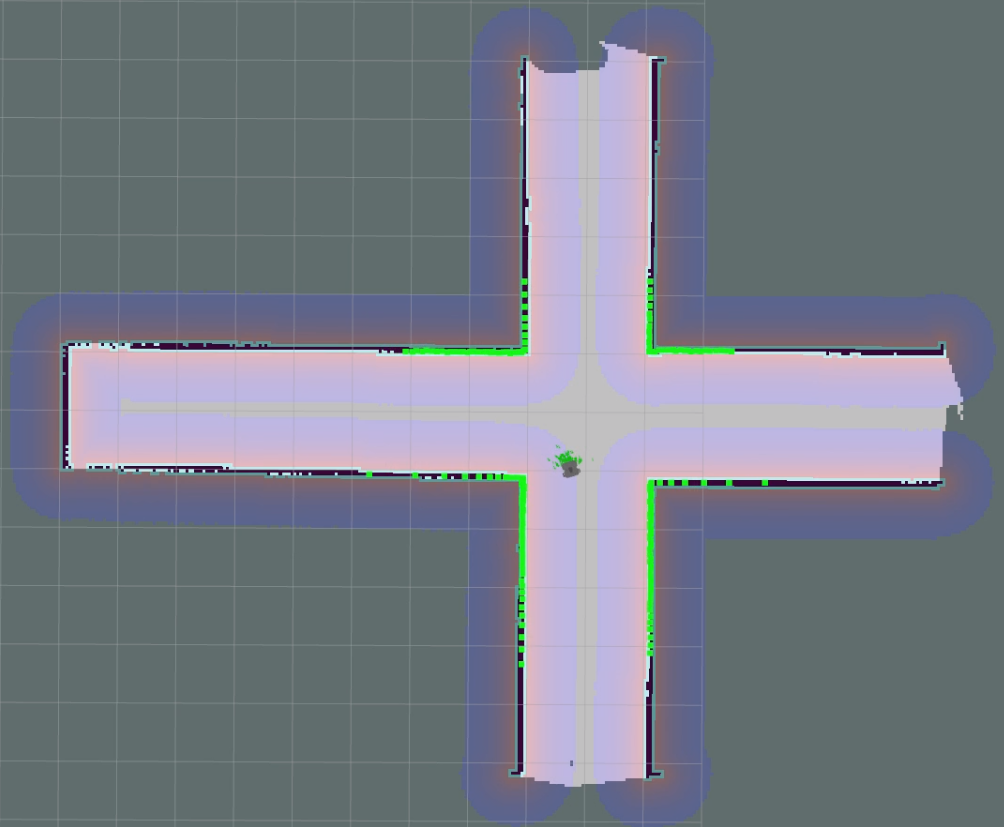
\includegraphics[width=\linewidth]{./figs/zyuzi_test_right.png}
      \subcaption{Test phase (target direction:turn right)}
      \label{exp1_test_right}
    \end{minipage}
  \end{tabular}
   \caption{State of the experiment}
   \label{fig::exp1_view}
\end{figure}
\newpage

\newpage
テストフェーズで,各経路を10回ずつ走行した結果をTable \ref{tb::exp1suc}に示す.
すべての経路において,目標地点へ到達することに成功した.
また,学習フェーズで収集したデータセットをFig. \ref{fig::exp1_result}に示す.
走行回数が多いContinueは突出しているが,それ以外の3つはほぼ同数であることが確認できる.
% \begin{table}[H]
%   \centering
%   \caption{Number of successes experiment 1 point}
%   \begin{tabular}{|c|c|}
%   \hline
%   Point & Number of successes \\ \hline
%   1     & 5/5                  \\ \hline
%   2     & 4/5                  \\ \hline
%   3     & 5/5                  \\ \hline
%   \end{tabular}
  
%   \label{tb::exp1suc}
%   \end{table}
\begin{table}[h]
  \caption{Number of successes experiment1}
  \label{tb::exp1suc}
  \begin{center}
      \vskip 0.5zh
      \begin{tabular}{|c|c|}
          \hline
          Route & Number of successes\\ \hline
          % Start - A (continue) & $10/10$ \\ \hline
          Start - A - B  & $10/10$ \\ \hline
          Start - A - C  & $10/10$ \\ \hline
          Start - A - D  & $10/10$ \\ \hline
      \end{tabular}
  \end{center}
\end{table}

\begin{figure}[ht]
  \centering
  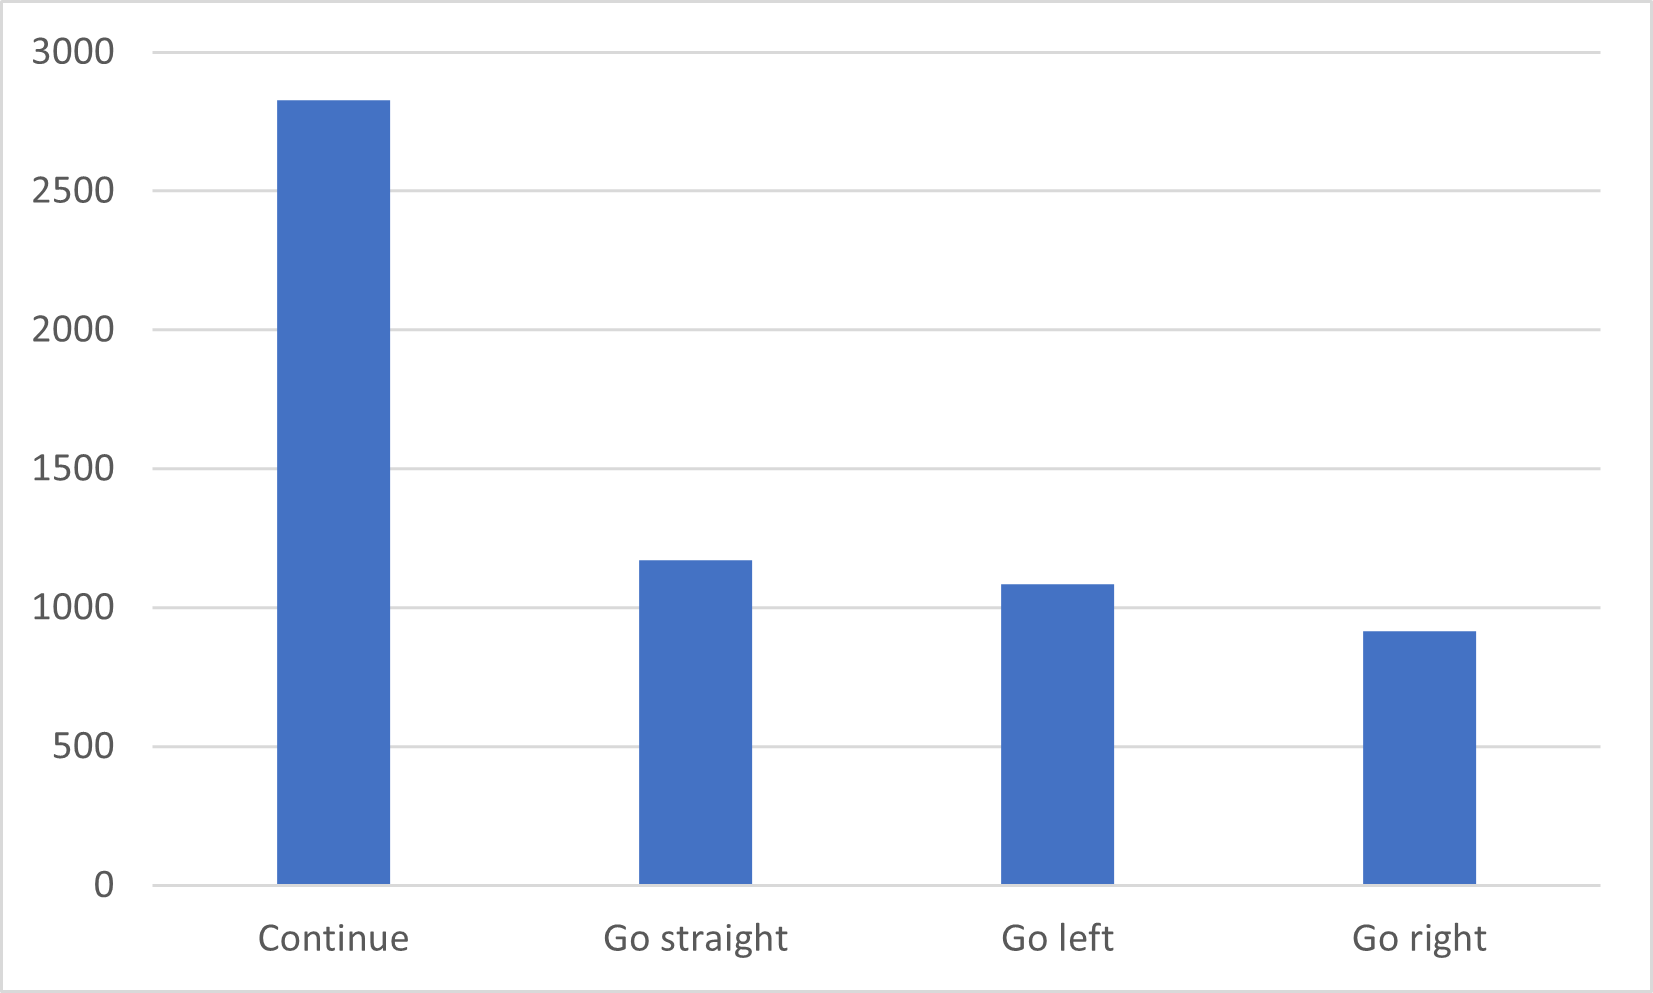
\includegraphics[width = 10cm]{./figs/exp1_result.png}
  \caption{Experiment1 dataset}
  \label{fig::exp1_result}
\end{figure}

\newpage
\section{実験2 (8の字コースを用いた実験)}
\subsection{実験目的}
実験1で用いた1つの十字路から環境を拡張し,
複雑な経路でも経路選択できるかを検証する.
% 提案手法を用いて,分岐路においてコマンドによってルートの変更が可能であるかさらなる検証を行う.
\subsection{実験環境}
Fig. \ref{fig::hatinozi}に示す.縦8[m]×横12[m]で道幅が2.5[m]の8の字型の環境を用いる.
この環境へロボットを青で示す初期位置,姿勢で配置する.
\begin{figure}[H]
    \centering
    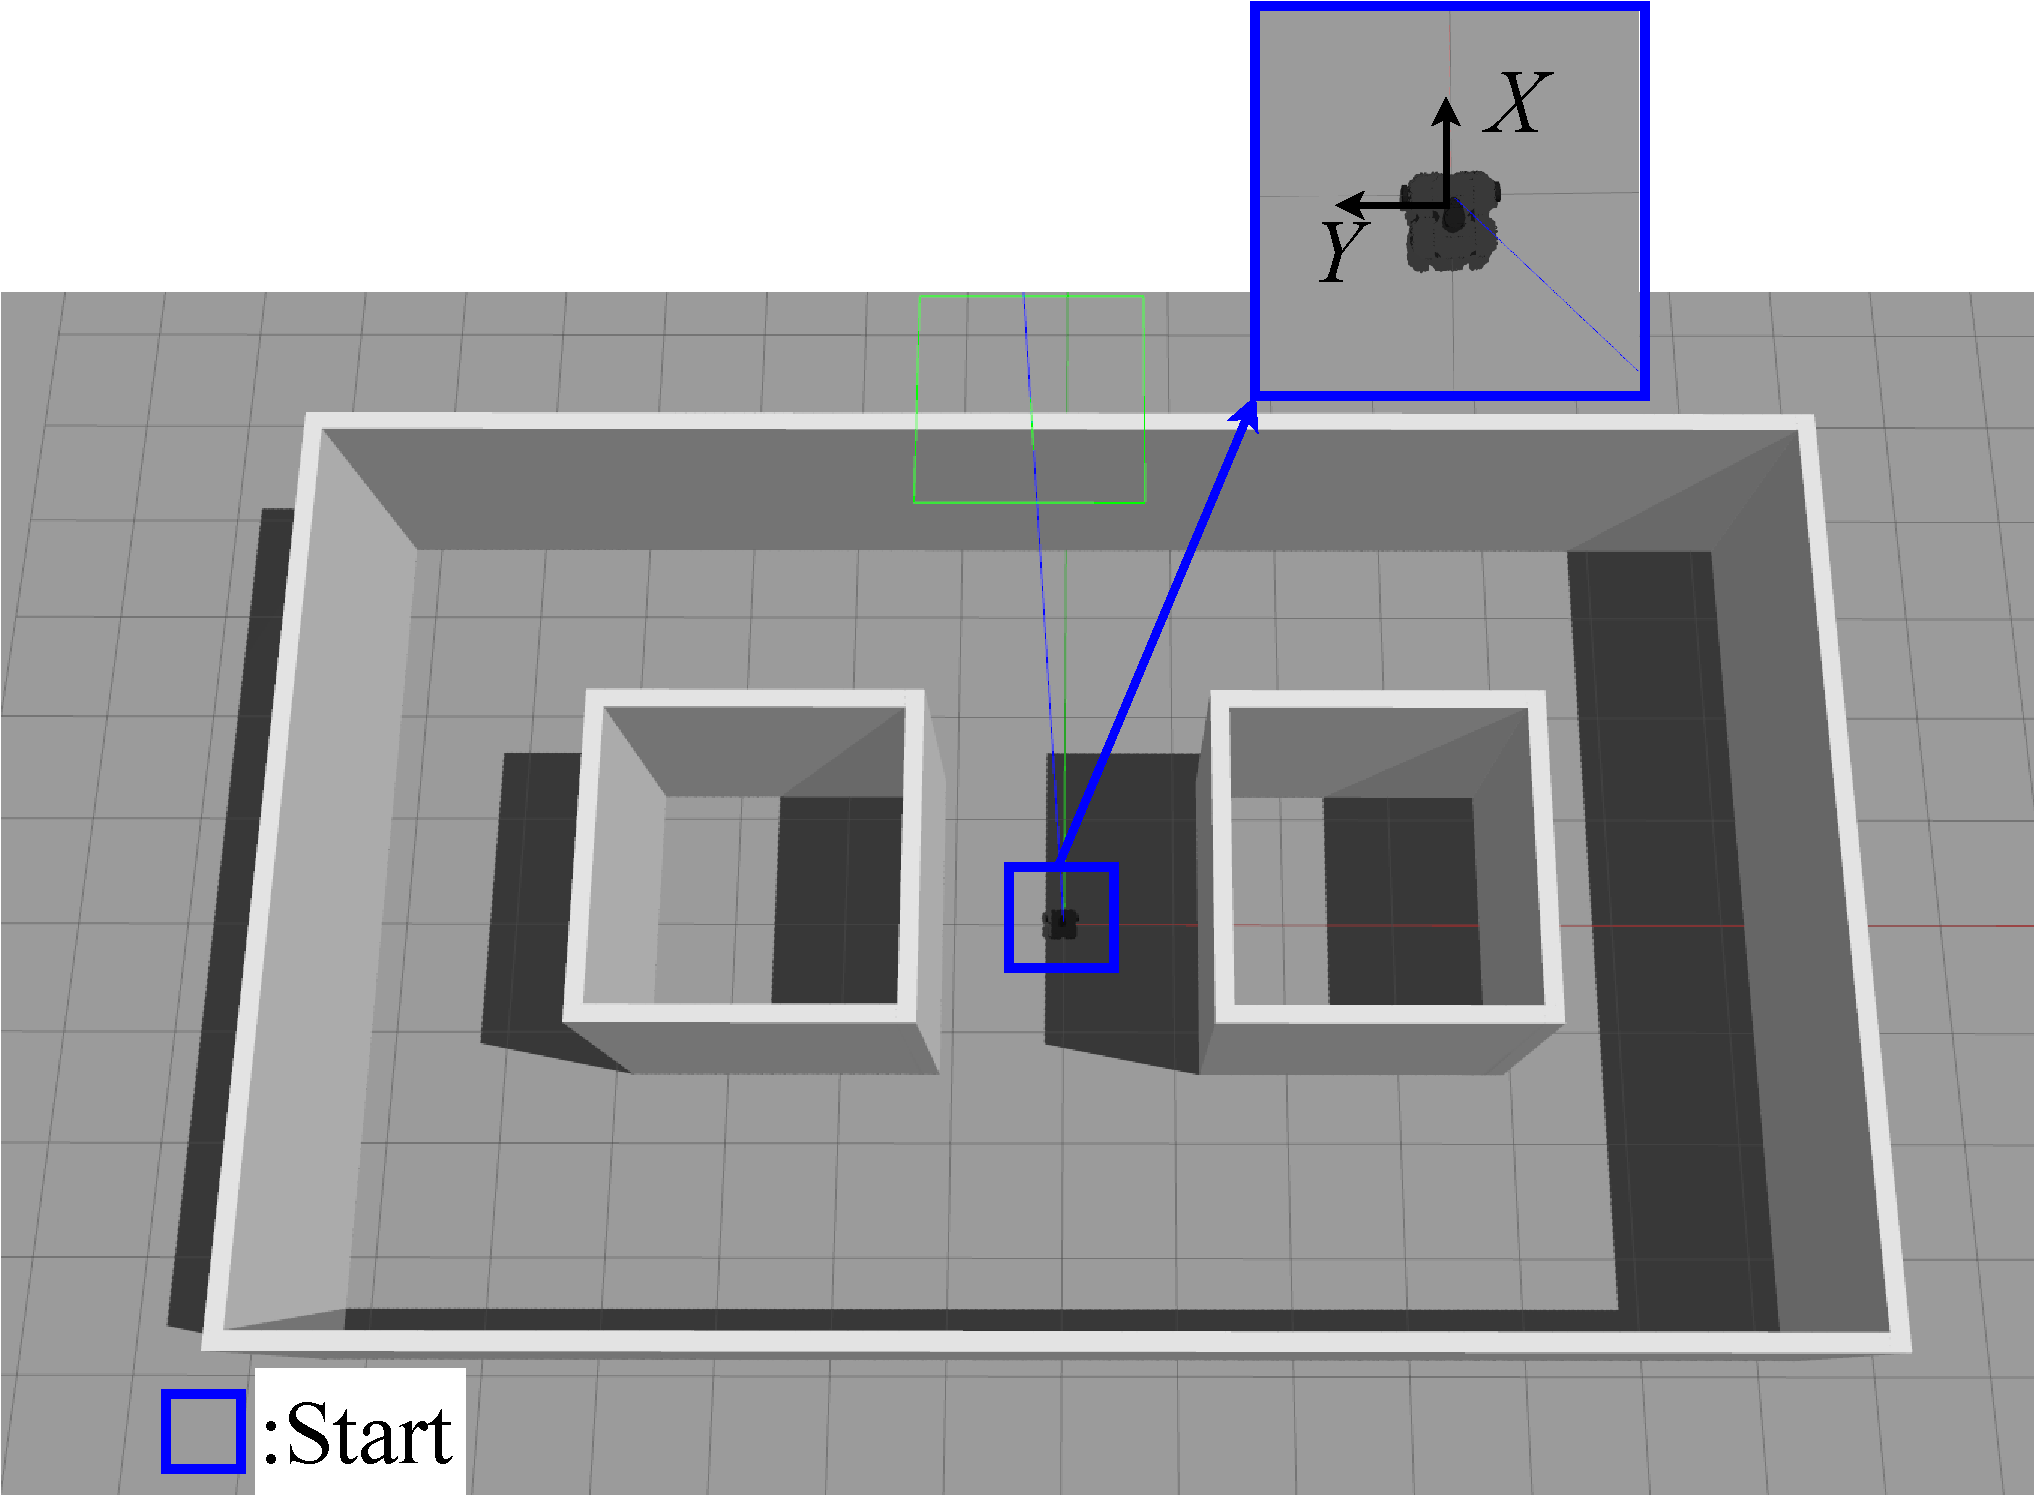
\includegraphics[width = 12cm]{./figs/coli.pdf}
    \caption{Experiment2 course}
    \label{fig::hatinozi}
\end{figure}

\newpage
Fig. \ref{fig::exp2route}に実験に用いる経路と,学習とテストで用いる目標方向指令を示す.
これらの環境を網羅するような経路を,
Route A-Fの順で60000[step]学習するまで,繰り返し走行する.
\begin{figure}[H]
    \begin{tabular}{cc}
      \begin{minipage}[t]{0.5\hsize}
        \centering
        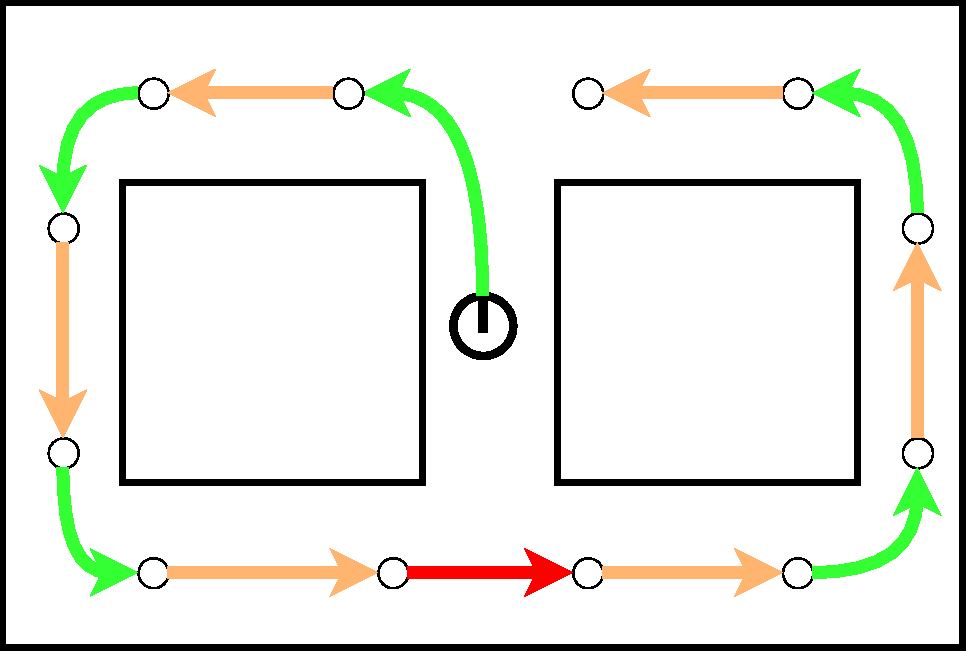
\includegraphics[keepaspectratio, scale=0.38]{./figs/8nozi_route-r1.pdf}
        \subcaption{Route A}
        \label{exp2route1}
      \end{minipage} 
      \begin{minipage}[t]{0.5\hsize}
        \centering
        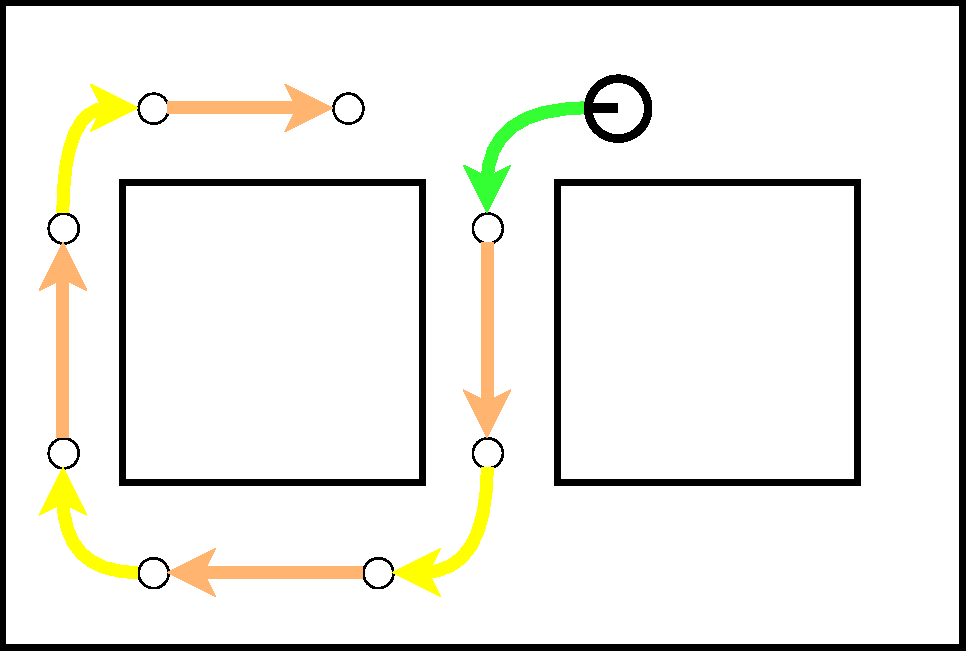
\includegraphics[keepaspectratio, scale=0.38]{./figs/8nozi_route-r2.pdf}
        \subcaption{Route B}
        \label{exp2route2}
      \end{minipage} \\
      \vspace{2.0zh}
      \begin{minipage}[t]{0.5\hsize}
        \centering
        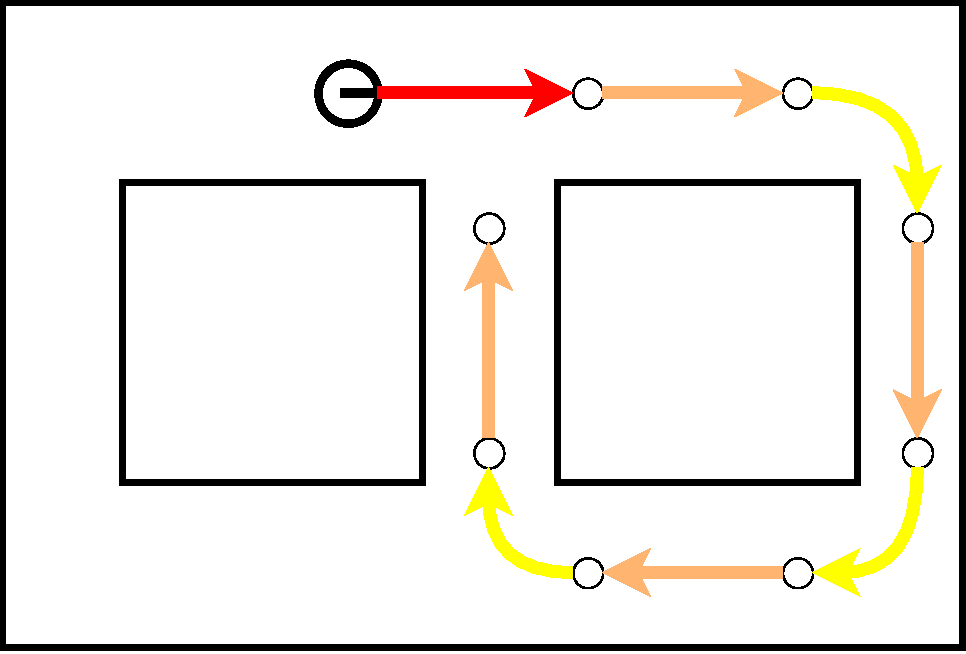
\includegraphics[keepaspectratio, scale=0.38]{./figs/8nozi_route-r3.pdf}
        \subcaption{Route C}
        \label{exp2route3}
      \end{minipage} 
      \begin{minipage}[t]{0.5\hsize}
        \centering
        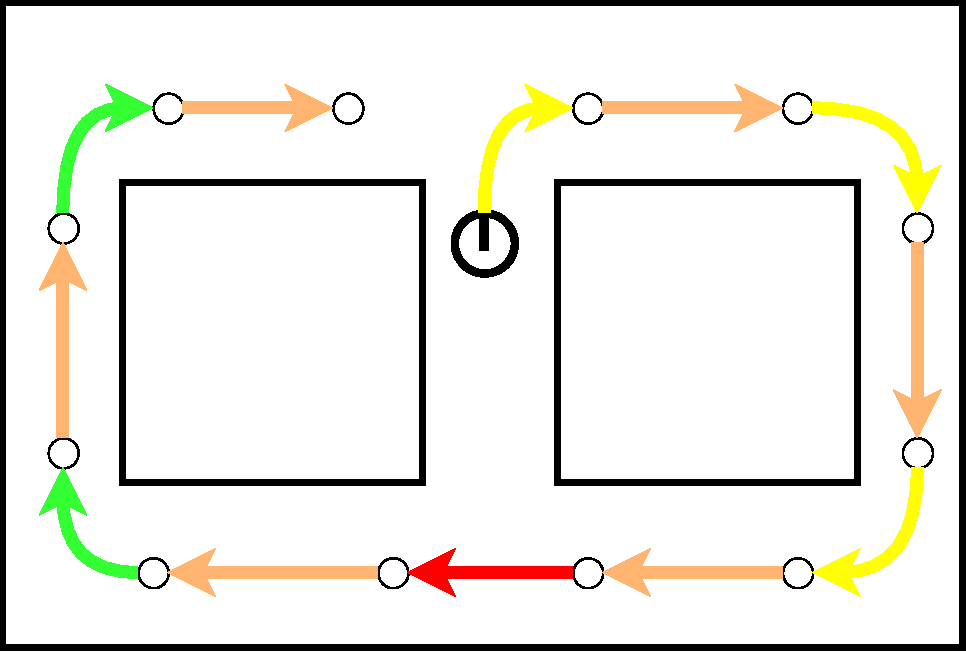
\includegraphics[keepaspectratio, scale=0.38]{./figs/8nozi_route-r4.pdf}
        \subcaption{Route D}
        \label{exp2route4}
      \end{minipage}\\

      \begin{minipage}[t]{0.5\hsize}
        \centering
        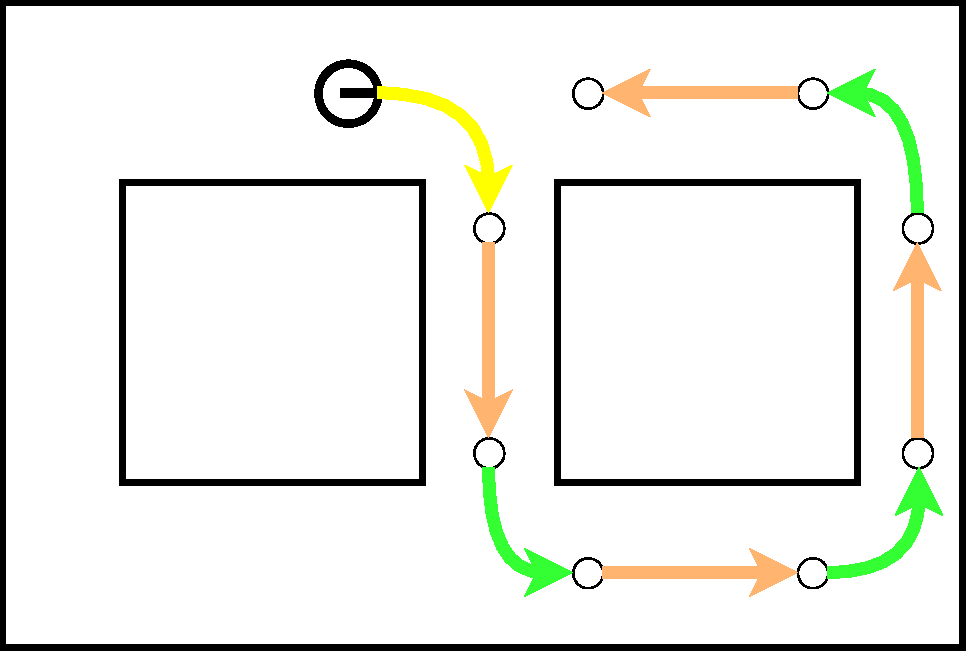
\includegraphics[keepaspectratio, scale=0.38]{./figs/8nozi_route-r5.pdf}
        \subcaption{Route E}
        \label{exp2route5}
      \end{minipage} 
      \begin{minipage}[t]{0.5\hsize}
        \centering
        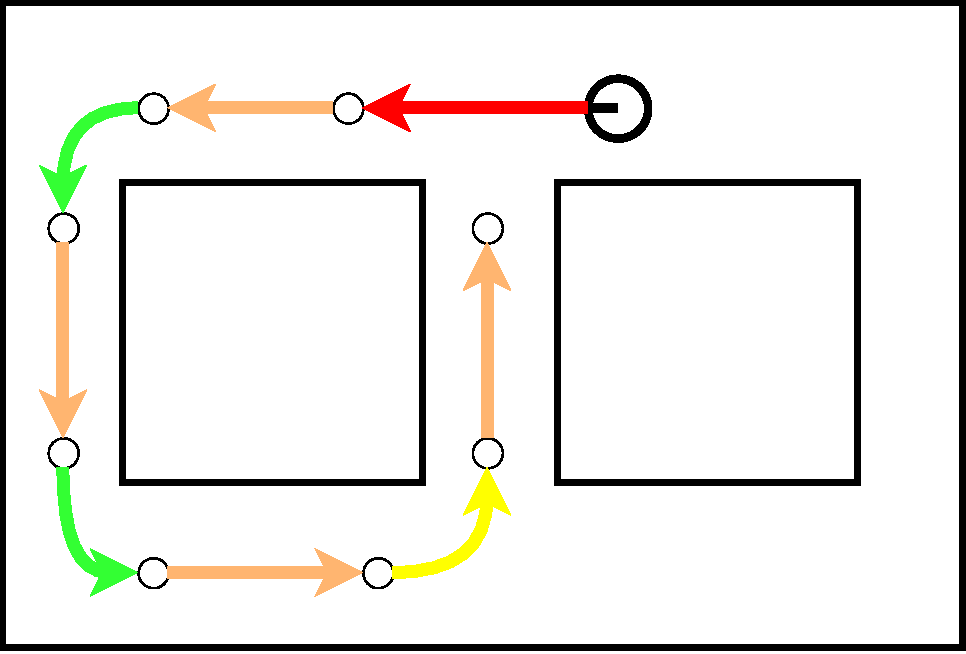
\includegraphics[keepaspectratio, scale=0.38]{./figs/8nozi_route-r6.pdf}
        \subcaption{Route F}
        \label{exp2route6}
      \end{minipage}
    \end{tabular}
    \begin{figure}[h]
      \centering
      
\includegraphics[width = 10cm]{./figs/8nizi_cap.pdf}
  \end{figure}
     \caption{Experiment 2 route}
     \label{fig::exp2route}
  \end{figure}
  
\newpage
\subsection{評価}
実験の様子をFig. \ref{fig::exp1_view}に示す.
Fig. \ref{exp1_ler_go}, \ref{exp1_ler_left}, \ref{exp1_ler_right}に示す学習フェーズでは,
赤で示した地図ベースの制御器による経路計画へ,追従するように走行する様子が確認できる.
また,Fig. \ref{exp1_test_go}, \ref{exp1_test_left}, \ref{exp1_test_right}に示すテストフェーズにおいて,
同一の分岐路で,目標方向により経路を選択する挙動が確認できる.
\begin{figure}[h]
  \begin{tabular}{cc}
    \begin{minipage}[t]{0.5\hsize}
      \centering
      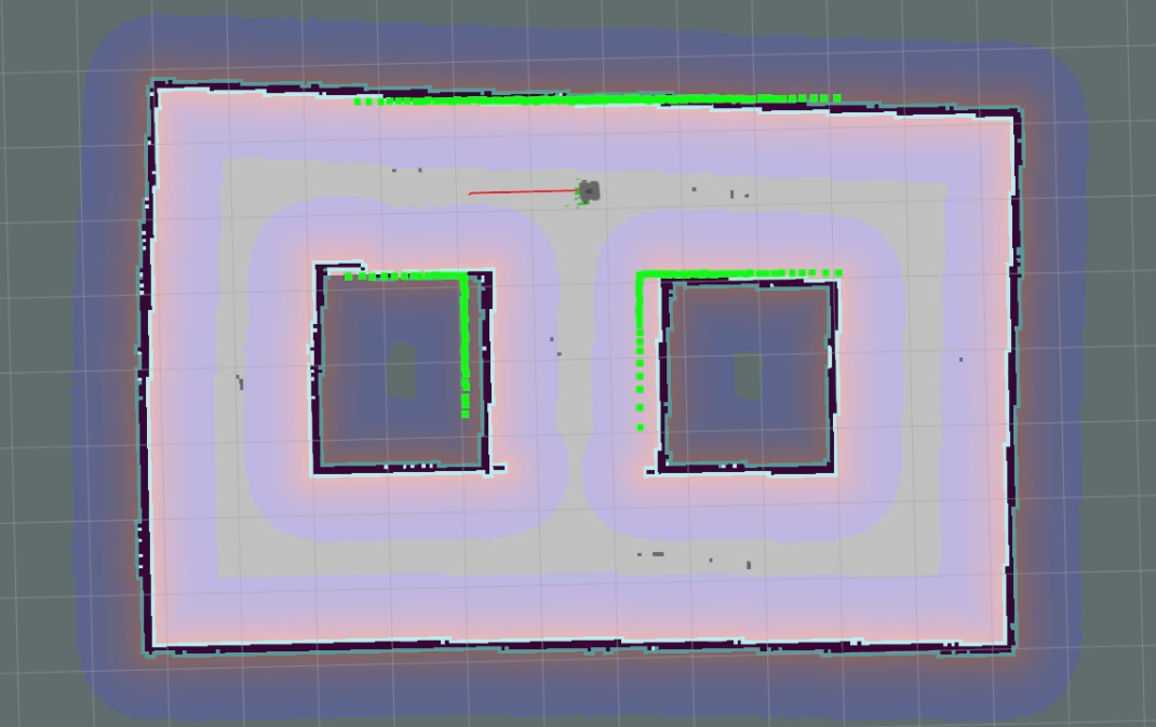
\includegraphics[height=4.3cm]{./figs/coli_ler_go.png}
      \subcaption{Learning phase (target direction:go straight)}
      \label{exp2_ler_go}
    \end{minipage} 
    \begin{minipage}[t]{0.5\hsize}
      \centering
      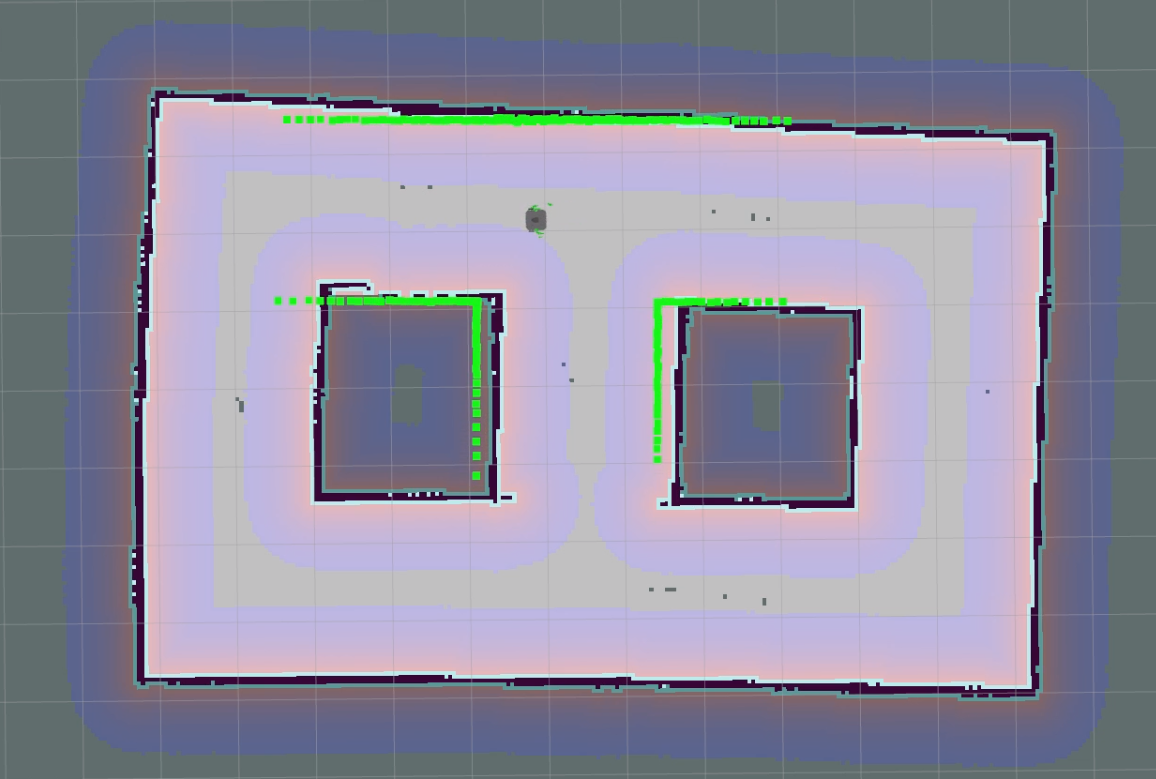
\includegraphics[height=4.3cm]{./figs/coli_test_go.png}
      \subcaption{Test phase (target direction:go straight)}
      \label{exp2_test_go}
    \end{minipage} \\
    \begin{minipage}[t]{0.5\hsize}
      \centering
      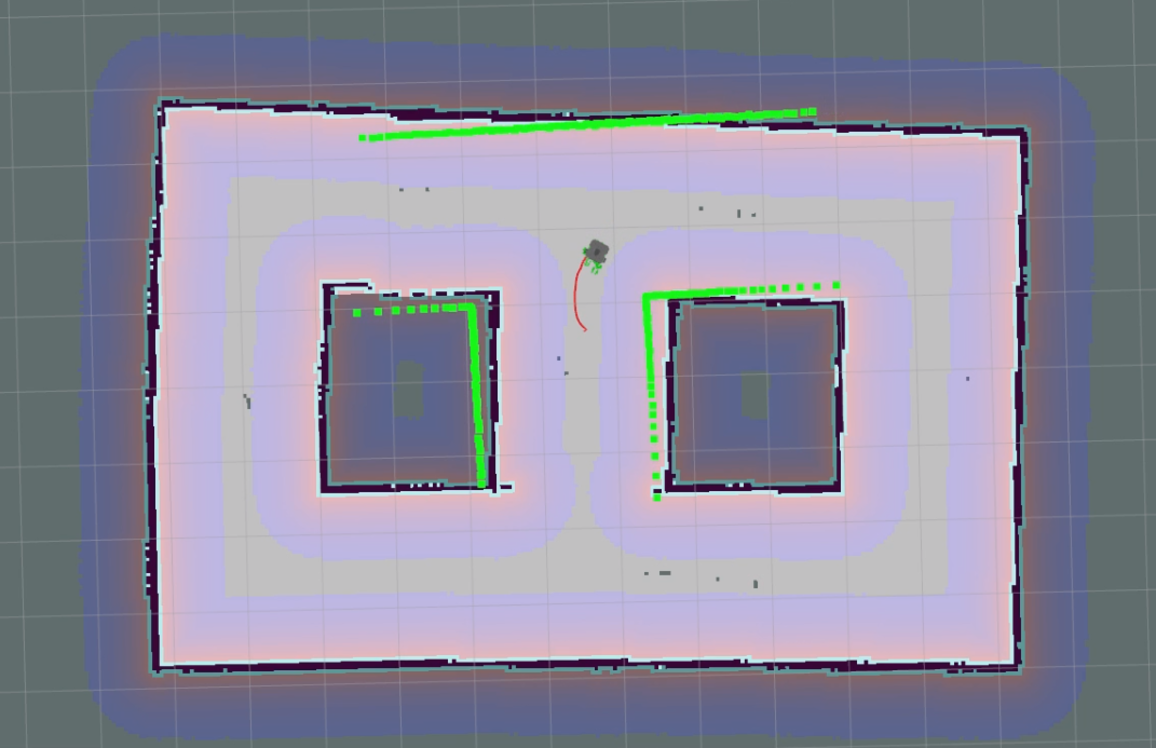
\includegraphics[height=4.4cm]{./figs/coli_ler_left.png}
      \subcaption{Learning phase (target direction:turn left)}
      \label{exp2_ler_left}
    \end{minipage} 
    \begin{minipage}[t]{0.5\hsize}
      \centering
      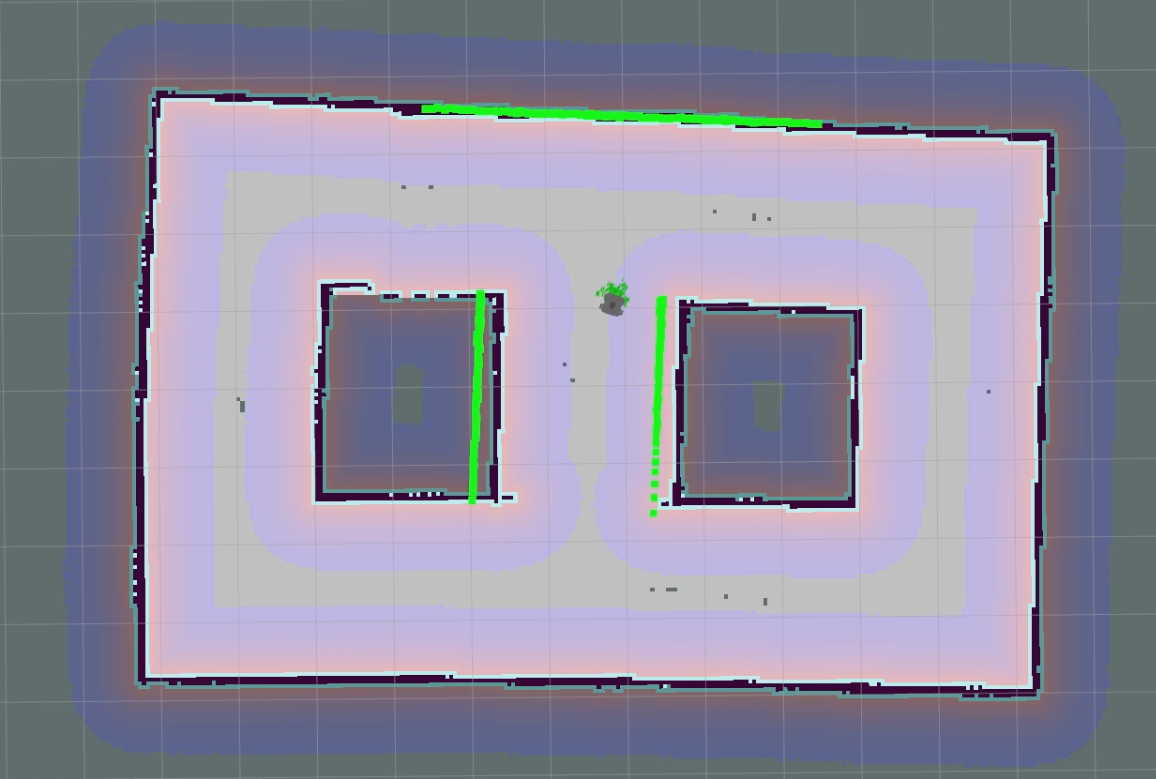
\includegraphics[height=4.4cm]{./figs/coli_test_left.png}
      \subcaption{Test phase (target direction:go turn left)}
      \label{exp2_test_left}
    \end{minipage} \\
  \end{tabular}
   \caption{State of the experiment2}
   \label{fig::exp2_view}
\end{figure}
\newpage
テストフェーズで,経路をランダムに60回走行を行った結果をTable \ref{tb::exp2suc}に示す.
結果として経路を約8割走行することに成功した.
また,学習フェーズで収集した目標方向指令のデータセットをFig. \ref{fig::exp2_result}に示す.
Go left,Go rightはほぼ同数であるが,Go straightは約半分以下となった.
しかし,Go straightを用いた,経路の選択は問題なく行うことができた.
これは,Go straightが学習する角速度が,Continueと類似しているからだと考えられる.
  \begin{table}[htb]
    \centering
    \caption{Number of successes experiment2}
    \begin{tabular}{|c|c|}
    \hline
    Route & Number of successes \\ \hline
    A-F     & 50/60                  \\ \hline
    \end{tabular}
    \label{tb::exp2suc}
    \vspace{2zh}
    \end{table} 
    \begin{figure}[ht]
      \centering
      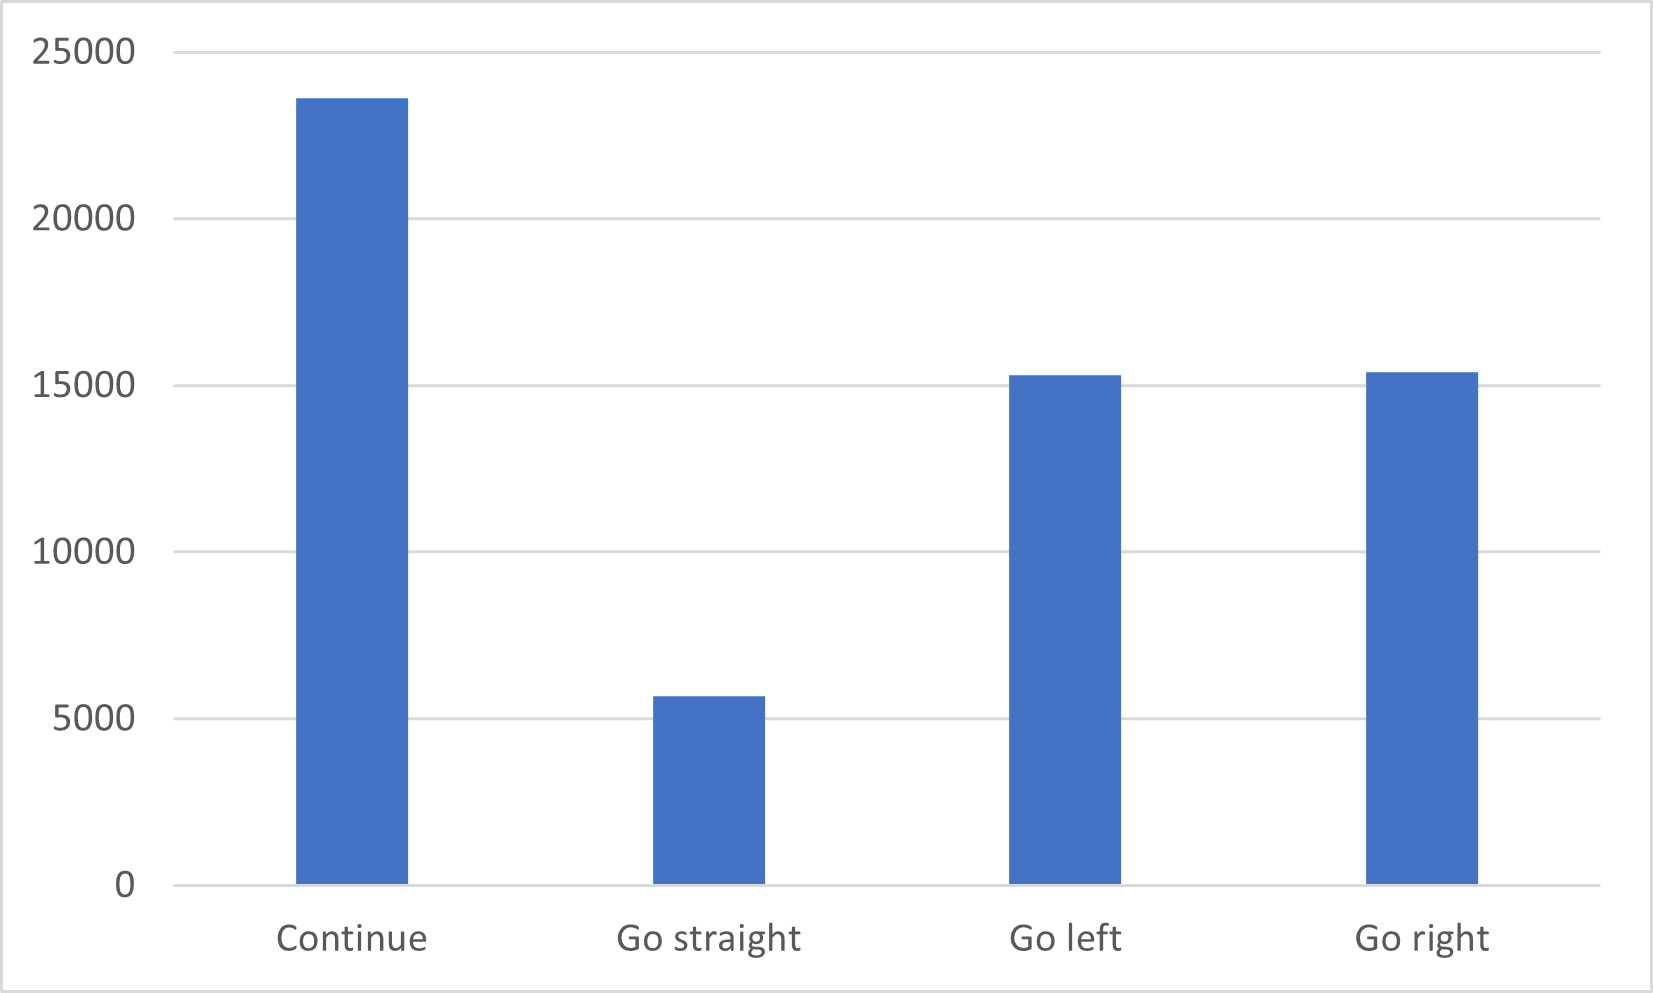
\includegraphics[width = 10cm]{./figs/exp2_result.png}
      \caption{Experiment2 dataset}
      \label{fig::exp2_result}
    \end{figure}
%結論
\chapter{結論}

本研究では,経路追従行動をカメラ画像を用いたend-to-end学習で模倣する
岡田ら\cite{okada}らの従来手法をベースに,データセットと学習器の入力へ目標方向を加えることで,
経路選択をする機能の追加を提案した.
またシミュレータ上で十字路,8の字の環境を用いた実験を行い,有効性の検証行った.
実験結果より,学習器へ目標方向を入力することで,経路選択が可能であることが示され,
提案手法の有効性が確認できた.
%謝辞
% \chapter*{謝辞}\addcontentsline{toc}{chapter}{謝辞}

熱心に指導されてくださった林原靖男教授
また先行研究や研究へのアドバイスなどの様々な面で,指導,サポートしてくださった
岡田眞也先輩,清岡優祐先輩.
私生活で精神面でのサポートをしていただいた蟹さん

母なる大地に感謝

%% Appendix
% \appendix{}
% %!TEX root = ../thesis.tex
\chapter*{付録}
\addcontentsline{toc}{chapter}{付録}
%
学習結果から得られた重みで, 移動ロボットにドリブルを行わせた際の様子を動画に記録した. 以下にYoutubeに投稿した動画のURLを載せる.\\
%
\vspace{3.0zh}\\
%
実験1の結果\\
\url{https://youtu.be/aTAcS6ppBog} \\
\vspace{1.0zh}\\
実験2の結果\\
\url{https://youtu.be/GLhenu6ki8o} \\
\vspace{1.0zh}\\
実験3の結果\\
\url{https://youtu.be/9-IQF1eQCwk} \\
\vspace{1.0zh}\\
実験4の結果\\
\url{https://youtu.be/RQocHlh2Bxk} \\
\vspace{1.0zh}\\

%
%% Back Matter
\backmatter{}
%
\maketitle
%
%!TEX root = ../thesis.tex
\chapter*{概要}
\thispagestyle{empty}
%
\begin{center}
  \scalebox{1.5}{カメラ画像と目標方向を用いたend-end学習による}\\
  \scalebox{1.5}{分岐路でのルート選択可能なのnavigation手法の提案}\\
\end{center}
\vspace{1.0zh}
%

近年,カメラ画像に基づいた自律移動の研究が行われている.
本研究室でも,LiDAR を用いた自律移動システムの出力を教師信号として与えることで
ロボットの経路追従行動をオンラインで模倣する手法を提案し,
実験により一定の経路を周回可能であると示されている.
本研究では,従来手法をベースに,目標とする進行方向("目標方向")をデータセットと学習器の入力へ加えることで,
分岐路で「直進」と「左折」などの経路を選択可能とする機能の追加を提案する.
提案手法では,LiDAR を用いた自律移動システムの出力をカメラ画像と目標方向を用いて模倣学習し,
学習後,カメラ画像と目標方向に基づいて経路を選択可能な自律走行を行う.
また,シミュレータを用いた実験により,提案手法の有効性を検証した. 

キーワード: end-to-end学習, Navigation, 目標方向
%
\newpage
%%
\chapter*{abstract}
\thispagestyle{empty}
%
\begin{center}
  \scalebox{1.3}{An End-to-End Navigation Method for Route Selection on Branch Roads}
  \scalebox{1.3}{Using Camera Images and Target Directions}\\
\end{center}
\vspace{1.0zh}
%

In recent years, research on autonomous mobility based on camera images has been conducted.
In our laboratory, we have proposed a method to imitate the path-following behavior of a robot online by providing the output of a LiDAR-based autonomous mobility system as a supervisory signal. I have also proposed a method to imitate the robot's path-following behavior online by providing the output of a LiDAR-based autonomous moving system as a supervisory signal, Experiments have shown that it is possible to follow a certain path.
In this study, based on the conventional method, I propose a method to imitate a robot's path-following behavior by adding a target direction ("target direction") to the data set and the input of the learner. 
In this paper, I propose to add a function that allows the user to select a path such as "straight ahead" or "left turn" at a forked road by adding the target direction ("target direction") to the dataset and the input of the learner.
The proposed method imitates and learns the output of a LiDAR-based autonomous mobility system using camera images and target directions.
After learning, the system runs autonomously and can select a route based on the camera image and the target direction.
I also verified the effectiveness of the proposed method by experiments using a simulator. 


keywords: End-to-end Learning, Navigation, Target Direction

%
\tableofcontents
%
\listoffigures
%
\listoftables
%

%

\end{document}
